% This file was converted to LaTeX by Writer2LaTeX ver. 1.4
% see http://writer2latex.sourceforge.net for more info
\documentclass[letterpaper]{article}
\usepackage[ascii]{inputenc}
\usepackage[T1]{fontenc}
\usepackage[english]{babel}
\usepackage{amsmath}
\usepackage{amssymb,amsfonts,textcomp}
\usepackage{color}
\usepackage{array}
\usepackage{supertabular}
\usepackage{hhline}
\usepackage{hyperref}
\hypersetup{pdftex, colorlinks=true, linkcolor=blue, citecolor=blue, filecolor=blue, urlcolor=blue, pdftitle=EE4: Circuit Board Design, pdfauthor=Derek, pdfsubject=Idea to schematic to board in 2 hours flat, pdfkeywords=}
\usepackage[pdftex]{graphicx}
% footnotes configuration
\makeatletter
\renewcommand\thefootnote{\arabic{footnote}}
\makeatother
% Text styles
\newcommand\textstyleSubtleEmphasis[1]{\textit{\textcolor[rgb]{0.5019608,0.5019608,0.5019608}{#1}}}
% Outline numbering
\setcounter{secnumdepth}{0}
\makeatletter
\newcommand\arraybslash{\let\\\@arraycr}
\makeatother
% List styles
\newcounter{saveenum}
\newcommand\liststyleRTFNumxvi{%
\renewcommand\labelitemi{{\textbullet}}
\renewcommand\labelitemii{o}
\renewcommand\labelitemiii{${\blacksquare}$}
\renewcommand\labelitemiv{{\textbullet}}
}
\newcommand\liststyleRTFNumix{%
\renewcommand\theenumi{\arabic{enumi}}
\renewcommand\theenumii{\alph{enumii}}
\renewcommand\theenumiii{\roman{enumiii}}
\renewcommand\theenumiv{\arabic{enumiv}}
\renewcommand\labelenumi{\theenumi.}
\renewcommand\labelenumii{\theenumii.}
\renewcommand\labelenumiii{\theenumiii.}
\renewcommand\labelenumiv{\theenumiv.}
}
\newcommand\liststyleRTFNumxiv{%
\renewcommand\labelitemi{{\textbullet}}
\renewcommand\labelitemii{o}
\renewcommand\labelitemiii{${\blacksquare}$}
\renewcommand\labelitemiv{{\textbullet}}
}
\newcommand\liststyleRTFNumvii{%
\renewcommand\labelitemi{{\textbullet}}
\renewcommand\labelitemii{o}
\renewcommand\labelitemiii{${\blacksquare}$}
\renewcommand\labelitemiv{{\textbullet}}
}
\newcommand\liststyleRTFNumvi{%
\renewcommand\theenumi{\arabic{enumi}}
\renewcommand\theenumii{\alph{enumii}}
\renewcommand\theenumiii{\roman{enumiii}}
\renewcommand\theenumiv{\arabic{enumiv}}
\renewcommand\labelenumi{\theenumi.}
\renewcommand\labelenumii{\theenumii.}
\renewcommand\labelenumiii{\theenumiii.}
\renewcommand\labelenumiv{\theenumiv.}
}
\newcommand\liststyleRTFNumxi{%
\renewcommand\theenumi{\arabic{enumi}}
\renewcommand\theenumii{\alph{enumii}}
\renewcommand\theenumiii{\roman{enumiii}}
\renewcommand\theenumiv{\arabic{enumiv}}
\renewcommand\labelenumi{\theenumi.}
\renewcommand\labelenumii{\theenumii.}
\renewcommand\labelenumiii{\theenumiii.}
\renewcommand\labelenumiv{\theenumiv.}
}
\newcommand\liststyleRTFNumxii{%
\renewcommand\labelitemi{{\textbullet}}
\renewcommand\labelitemii{o}
\renewcommand\labelitemiii{${\blacksquare}$}
\renewcommand\labelitemiv{{\textbullet}}
}
\newcommand\liststyleRTFNumxv{%
\renewcommand\labelitemi{{\textbullet}}
\renewcommand\labelitemii{o}
\renewcommand\labelitemiii{${\blacksquare}$}
\renewcommand\labelitemiv{{\textbullet}}
}
\newcommand\liststyleRTFNumxvii{%
\renewcommand\labelitemi{{\textbullet}}
\renewcommand\labelitemii{o}
\renewcommand\labelitemiii{${\blacksquare}$}
\renewcommand\labelitemiv{{\textbullet}}
}
\newcommand\liststyleRTFNumiv{%
\renewcommand\labelitemi{{\textbullet}}
\renewcommand\labelitemii{o}
\renewcommand\labelitemiii{${\blacksquare}$}
\renewcommand\labelitemiv{{\textbullet}}
}
\newcommand\liststyleRTFNumiii{%
\renewcommand\labelitemi{{\textbullet}}
\renewcommand\labelitemii{o}
\renewcommand\labelitemiii{${\blacksquare}$}
\renewcommand\labelitemiv{{\textbullet}}
}
% Page layout (geometry)
\setlength\voffset{-1in}
\setlength\hoffset{-1in}
\setlength\topmargin{0.25in}
\setlength\oddsidemargin{0.5in}
\setlength\textheight{7.827999in}
\setlength\textwidth{7.5in}
\setlength\footskip{0.96099997in}
\setlength\headheight{0.75in}
\setlength\headsep{0.711in}
% Footnote rule
\setlength{\skip\footins}{0.0469in}
\renewcommand\footnoterule{\vspace*{-0.0071in}\setlength\leftskip{0pt}\setlength\rightskip{0pt plus 1fil}\noindent\textcolor{black}{\rule{0.25\columnwidth}{0.0071in}}\vspace*{0.0398in}}
% Pages styles
\makeatletter
\newcommand\ps@Standard{
  \renewcommand\@oddhead{[Warning: Draw object ignored]}
  \renewcommand\@evenhead{}
  \renewcommand\@oddfoot{}
  \renewcommand\@evenfoot{}
  \renewcommand\thepage{\arabic{page}}
}
\makeatother
\pagestyle{Standard}
\setlength\tabcolsep{1mm}
\renewcommand\arraystretch{1.3}
\title{EE4: Circuit Board Design}
\author{Derek}
\date{2016-09-10}
\begin{document}
\clearpage\setcounter{page}{1}\pagestyle{Standard}
{\centering\selectlanguage{english}\sffamily\bfseries\color[rgb]{0.30980393,0.5058824,0.7411765}
EE4: Circuit Board Design
\par}

{\centering\selectlanguage{english}\itshape\color[rgb]{0.30980393,0.5058824,0.7411765}
Idea to schematic to board in 2 hours flat
\par}

{\centering\selectlanguage{english}\itshape\color[rgb]{0.30980393,0.5058824,0.7411765}
\textstyleSubtleEmphasis{\textup{Richard ``Ducky'' Lin}}
\par}


\bigskip

{\selectlanguage{english}\sffamily\color[rgb]{0.30980393,0.5058824,0.7411765}
\textbf{Application:} You've designed and prototyped circuits. But you never see a finished product on a breadboard -
rather, they are almost always on a custom circuit board. Now, you will learn how to design these boards.}

\section{Table of Contents}
{\selectlanguage{english}\sffamily\color[rgb]{0.30980393,0.5058824,0.7411765}
\hyperlink{Toc337742671}{\textcolor{blue}{Introduction\ \ }}}

{\selectlanguage{english}\sffamily\color[rgb]{0.30980393,0.5058824,0.7411765}
\hyperlink{Toc337742672}{\textcolor{blue}{Technical Manual\ \ }}}

{\selectlanguage{english}\sffamily\color[rgb]{0.30980393,0.5058824,0.7411765}
\hyperlink{Toc337742673}{\textcolor{blue}{What is a printed circuit board?\ \ }}}

{\selectlanguage{english}\sffamily\color[rgb]{0.30980393,0.5058824,0.7411765}
\hyperlink{Toc337742674}{\textcolor{blue}{Anatomy of a printed circuit board\ \ }}}

{\selectlanguage{english}\sffamily\color[rgb]{0.30980393,0.5058824,0.7411765}
\hyperlink{Toc337742675}{\textcolor{blue}{Electronic design automation (EDA)\ \ }}}

{\selectlanguage{english}\sffamily\color[rgb]{0.30980393,0.5058824,0.7411765}
\hyperlink{Toc337742676}{\textcolor{blue}{Workflow overview\ \ }}}

{\selectlanguage{english}\sffamily\color[rgb]{0.30980393,0.5058824,0.7411765}
\hyperlink{Toc337742677}{\textcolor{blue}{Schematic capture\ \ }}}

{\selectlanguage{english}\sffamily\color[rgb]{0.30980393,0.5058824,0.7411765}
\hyperlink{Toc337742678}{\textcolor{blue}{Components\ \ }}}

{\selectlanguage{english}\sffamily\color[rgb]{0.30980393,0.5058824,0.7411765}
\hyperlink{Toc337742679}{\textcolor{blue}{Basic concepts\ \ }}}

{\selectlanguage{english}\sffamily\color[rgb]{0.30980393,0.5058824,0.7411765}
\hyperlink{Toc337742680}{\textcolor{blue}{Good practices\ \ }}}

{\selectlanguage{english}\sffamily\color[rgb]{0.30980393,0.5058824,0.7411765}
\hyperlink{Toc337742681}{\textcolor{blue}{Board layout\ \ }}}

{\selectlanguage{english}\sffamily\color[rgb]{0.30980393,0.5058824,0.7411765}
\hyperlink{Toc337742682}{\textcolor{blue}{Basic concepts\ \ }}}

{\selectlanguage{english}\sffamily\color[rgb]{0.30980393,0.5058824,0.7411765}
\hyperlink{Toc337742683}{\textcolor{blue}{Design rules\ \ }}}

{\selectlanguage{english}\sffamily\color[rgb]{0.30980393,0.5058824,0.7411765}
\hyperlink{Toc337742684}{\textcolor{blue}{Practical considerations\ \ }}}

{\selectlanguage{english}\sffamily\color[rgb]{0.30980393,0.5058824,0.7411765}
\hyperlink{Toc337742685}{\textcolor{blue}{Good practices\ \ }}}

{\selectlanguage{english}\sffamily\color[rgb]{0.30980393,0.5058824,0.7411765}
\hyperlink{Toc337742686}{\textcolor{blue}{Fabrication\ \ }}}

{\selectlanguage{english}\sffamily\color[rgb]{0.30980393,0.5058824,0.7411765}
\hyperlink{Toc337742687}{\textcolor{blue}{Verification \& design rule checking (DRC)\ \ }}}

{\selectlanguage{english}\sffamily\color[rgb]{0.30980393,0.5058824,0.7411765}
\hyperlink{Toc337742688}{\textcolor{blue}{Gerbers\ \ }}}

{\selectlanguage{english}\sffamily\color[rgb]{0.30980393,0.5058824,0.7411765}
\hyperlink{Toc337742689}{\textcolor{blue}{Assembly\ \ }}}

{\selectlanguage{english}\sffamily\color[rgb]{0.30980393,0.5058824,0.7411765}
\hyperlink{Toc337742690}{\textcolor{blue}{Advanced: Component creation\ \ }}}

{\selectlanguage{english}\sffamily\color[rgb]{0.30980393,0.5058824,0.7411765}
\hyperlink{Toc337742691}{\textcolor{blue}{Schematic Symbols\ \ }}}

{\selectlanguage{english}\sffamily\color[rgb]{0.30980393,0.5058824,0.7411765}
\hyperlink{Toc337742692}{\textcolor{blue}{Component footprints / patterns\ \ }}}

{\selectlanguage{english}\sffamily\color[rgb]{0.30980393,0.5058824,0.7411765}
\hyperlink{Toc337742693}{\textcolor{blue}{Parts List\ \ }}}

{\selectlanguage{english}\sffamily\color[rgb]{0.30980393,0.5058824,0.7411765}
\hyperlink{Toc337742694}{\textcolor{blue}{Lab Manual\ \ }}}

{\selectlanguage{english}\sffamily\color[rgb]{0.30980393,0.5058824,0.7411765}
\hyperlink{Toc337742695}{\textcolor{blue}{Lab 3.0: Pre-lab: setup and circuit overview\ \ }}}

{\selectlanguage{english}\sffamily\color[rgb]{0.30980393,0.5058824,0.7411765}
\hyperlink{Toc337742696}{\textcolor{blue}{Lab 3.1: Circuit design\ \ }}}

{\selectlanguage{english}\sffamily\color[rgb]{0.30980393,0.5058824,0.7411765}
\hyperlink{Toc337742697}{\textcolor{blue}{Lab 3.2: Schematic entry\ \ }}}

{\selectlanguage{english}\sffamily\color[rgb]{0.30980393,0.5058824,0.7411765}
\hyperlink{Toc337742698}{\textcolor{blue}{Lab 3.3: Layout\ \ }}}

{\selectlanguage{english}\sffamily\color[rgb]{0.30980393,0.5058824,0.7411765}
\hyperlink{Toc337742699}{\textcolor{blue}{Lab 3.4: Forward annotation\ \ }}}

{\selectlanguage{english}\sffamily\color[rgb]{0.30980393,0.5058824,0.7411765}
\hyperlink{Toc337742700}{\textcolor{blue}{Lab 3.5: Design verification\ \ }}}

{\selectlanguage{english}\sffamily\color[rgb]{0.30980393,0.5058824,0.7411765}
\hyperlink{Toc337742701}{\textcolor{blue}{Lab 3.6: Fabrication data\ \ }}}

{\selectlanguage{english}\sffamily\color[rgb]{0.30980393,0.5058824,0.7411765}
\hyperlink{Toc337742702}{\textcolor{blue}{Lab 3.7: Extra for Experts: Component creation \& surface mount\ \ }}}

{\selectlanguage{english}\sffamily\color[rgb]{0.30980393,0.5058824,0.7411765}
\hyperlink{Toc337742703}{\textcolor{blue}{Pattern creation\ \ }}}

{\selectlanguage{english}\sffamily\color[rgb]{0.30980393,0.5058824,0.7411765}
\hyperlink{Toc337742704}{\textcolor{blue}{Component creation\ \ }}}

{\selectlanguage{english}\sffamily\color[rgb]{0.30980393,0.5058824,0.7411765}
\hyperlink{Toc337742705}{\textcolor{blue}{Revising the schematic\ \ }}}

{\selectlanguage{english}\sffamily\color[rgb]{0.30980393,0.5058824,0.7411765}
\hyperlink{Toc337742706}{\textcolor{blue}{Revising the board\ \ }}}

{\selectlanguage{english}\sffamily\color[rgb]{0.30980393,0.5058824,0.7411765}
\hyperlink{Toc337742707}{\textcolor{blue}{Design Software\ \ }}}

{\selectlanguage{english}\sffamily\color[rgb]{0.30980393,0.5058824,0.7411765}
\hyperlink{Toc337742708}{\textcolor{blue}{Free \& Open Source\ \ }}}

{\selectlanguage{english}\sffamily\color[rgb]{0.30980393,0.5058824,0.7411765}
\hyperlink{Toc337742709}{\textcolor{blue}{Commercial\ \ }}}

{\selectlanguage{english}\sffamily\color[rgb]{0.30980393,0.5058824,0.7411765}
\hyperlink{Toc337742710}{\textcolor{blue}{Software you can afford\ \ }}}

{\selectlanguage{english}\sffamily\color[rgb]{0.30980393,0.5058824,0.7411765}
\hyperlink{Toc337742711}{\textcolor{blue}{Software for the 1\%\ \ }}}

{\selectlanguage{english}\sffamily\color[rgb]{0.30980393,0.5058824,0.7411765}
\hyperlink{Toc337742712}{\textcolor{blue}{PCBs and You\ \ }}}

{\selectlanguage{english}\sffamily\color[rgb]{0.30980393,0.5058824,0.7411765}
\hyperlink{Toc337742713}{\textcolor{blue}{Advanced Circuits\ \ }}}

{\selectlanguage{english}\sffamily\color[rgb]{0.30980393,0.5058824,0.7411765}
\hyperlink{Toc337742714}{\textcolor{blue}{BatchPCB\ \ }}}

{\selectlanguage{english}\sffamily\color[rgb]{0.30980393,0.5058824,0.7411765}
\hyperlink{Toc337742715}{\textcolor{blue}{Dorkbot PDX / OSH Park\ \ }}}

{\selectlanguage{english}\sffamily\color[rgb]{0.30980393,0.5058824,0.7411765}
\hyperlink{Toc337742716}{\textcolor{blue}{SeeedStudio\ \ }}}

{\selectlanguage{english}\sffamily\color[rgb]{0.30980393,0.5058824,0.7411765}
\hyperlink{Toc337742717}{\textcolor{blue}{Sources \& Further Reading\ \ }}}


\bigskip

\clearpage
\bigskip

\section{Revision History}
\begin{flushleft}
\tablefirsthead{}
\tablehead{}
\tabletail{}
\tablelasttail{}
\begin{supertabular}{|m{0.9900598in}|m{0.9136598in}|m{5.3670597in}|}
\hline
{\selectlanguage{english}\sffamily\bfseries\color[rgb]{0.30980393,0.5058824,0.7411765} Version} &
{\selectlanguage{english}\sffamily\bfseries\color[rgb]{0.30980393,0.5058824,0.7411765} Date} &
{\selectlanguage{english}\sffamily\bfseries\color[rgb]{0.30980393,0.5058824,0.7411765} Changelist}\\\hline
{\selectlanguage{english}\sffamily\color[rgb]{0.30980393,0.5058824,0.7411765} 1.0} &
{\selectlanguage{english}\sffamily\color[rgb]{0.30980393,0.5058824,0.7411765} Fall 2011} &
{\selectlanguage{english}\sffamily\color[rgb]{0.30980393,0.5058824,0.7411765} Initial release}\\\hline
{\selectlanguage{english}\sffamily\color[rgb]{0.30980393,0.5058824,0.7411765} 1.1} &
{\selectlanguage{english}\sffamily\color[rgb]{0.30980393,0.5058824,0.7411765} 11 Oct 2012} &
{\selectlanguage{english}\sffamily\color[rgb]{0.30980393,0.5058824,0.7411765} Various typo fixes and clarifications}

{\selectlanguage{english}\sffamily\color[rgb]{0.30980393,0.5058824,0.7411765} Expanded section on good
practices}\\\hline
\end{supertabular}
\end{flushleft}
\section{Licensing}
 
\includegraphics[width=0.9165in,height=0.3228in]{figures/ee4document-img001.png} 

{\selectlanguage{english}\sffamily\color[rgb]{0.30980393,0.5058824,0.7411765}
This document (including source elements, like diagrams), is licensed under the Creative Commons Attribution-ShareAlike
3.0 Unported License (\url{http://creativecommons.org/licenses/by-sa/3.0/deed.en_US}).}


\bigskip

{\selectlanguage{english}\sffamily\color[rgb]{0.30980393,0.5058824,0.7411765}
While commercial use is not prohibited under the terms of the license (the drawbacks outweigh the benefits, nor is a
solar car team going to start suing people for obscene amounts over copyright infringement), you shouldn't be
shamelessly trying to turn a profit off someone else's work. What exactly this means is completely up to you -- but
please behave like responsible adults. Keep in mind that you must license any derivative works under a similar license
-- which gives recipients redistribution rights.}

\clearpage
\bigskip

\section{Introduction}
{\selectlanguage{english}\sffamily\color[rgb]{0.30980393,0.5058824,0.7411765}
In the previous labs, you've been introduced to basic circuit design, and have even prototyped them on a solderless
breadboard.}

 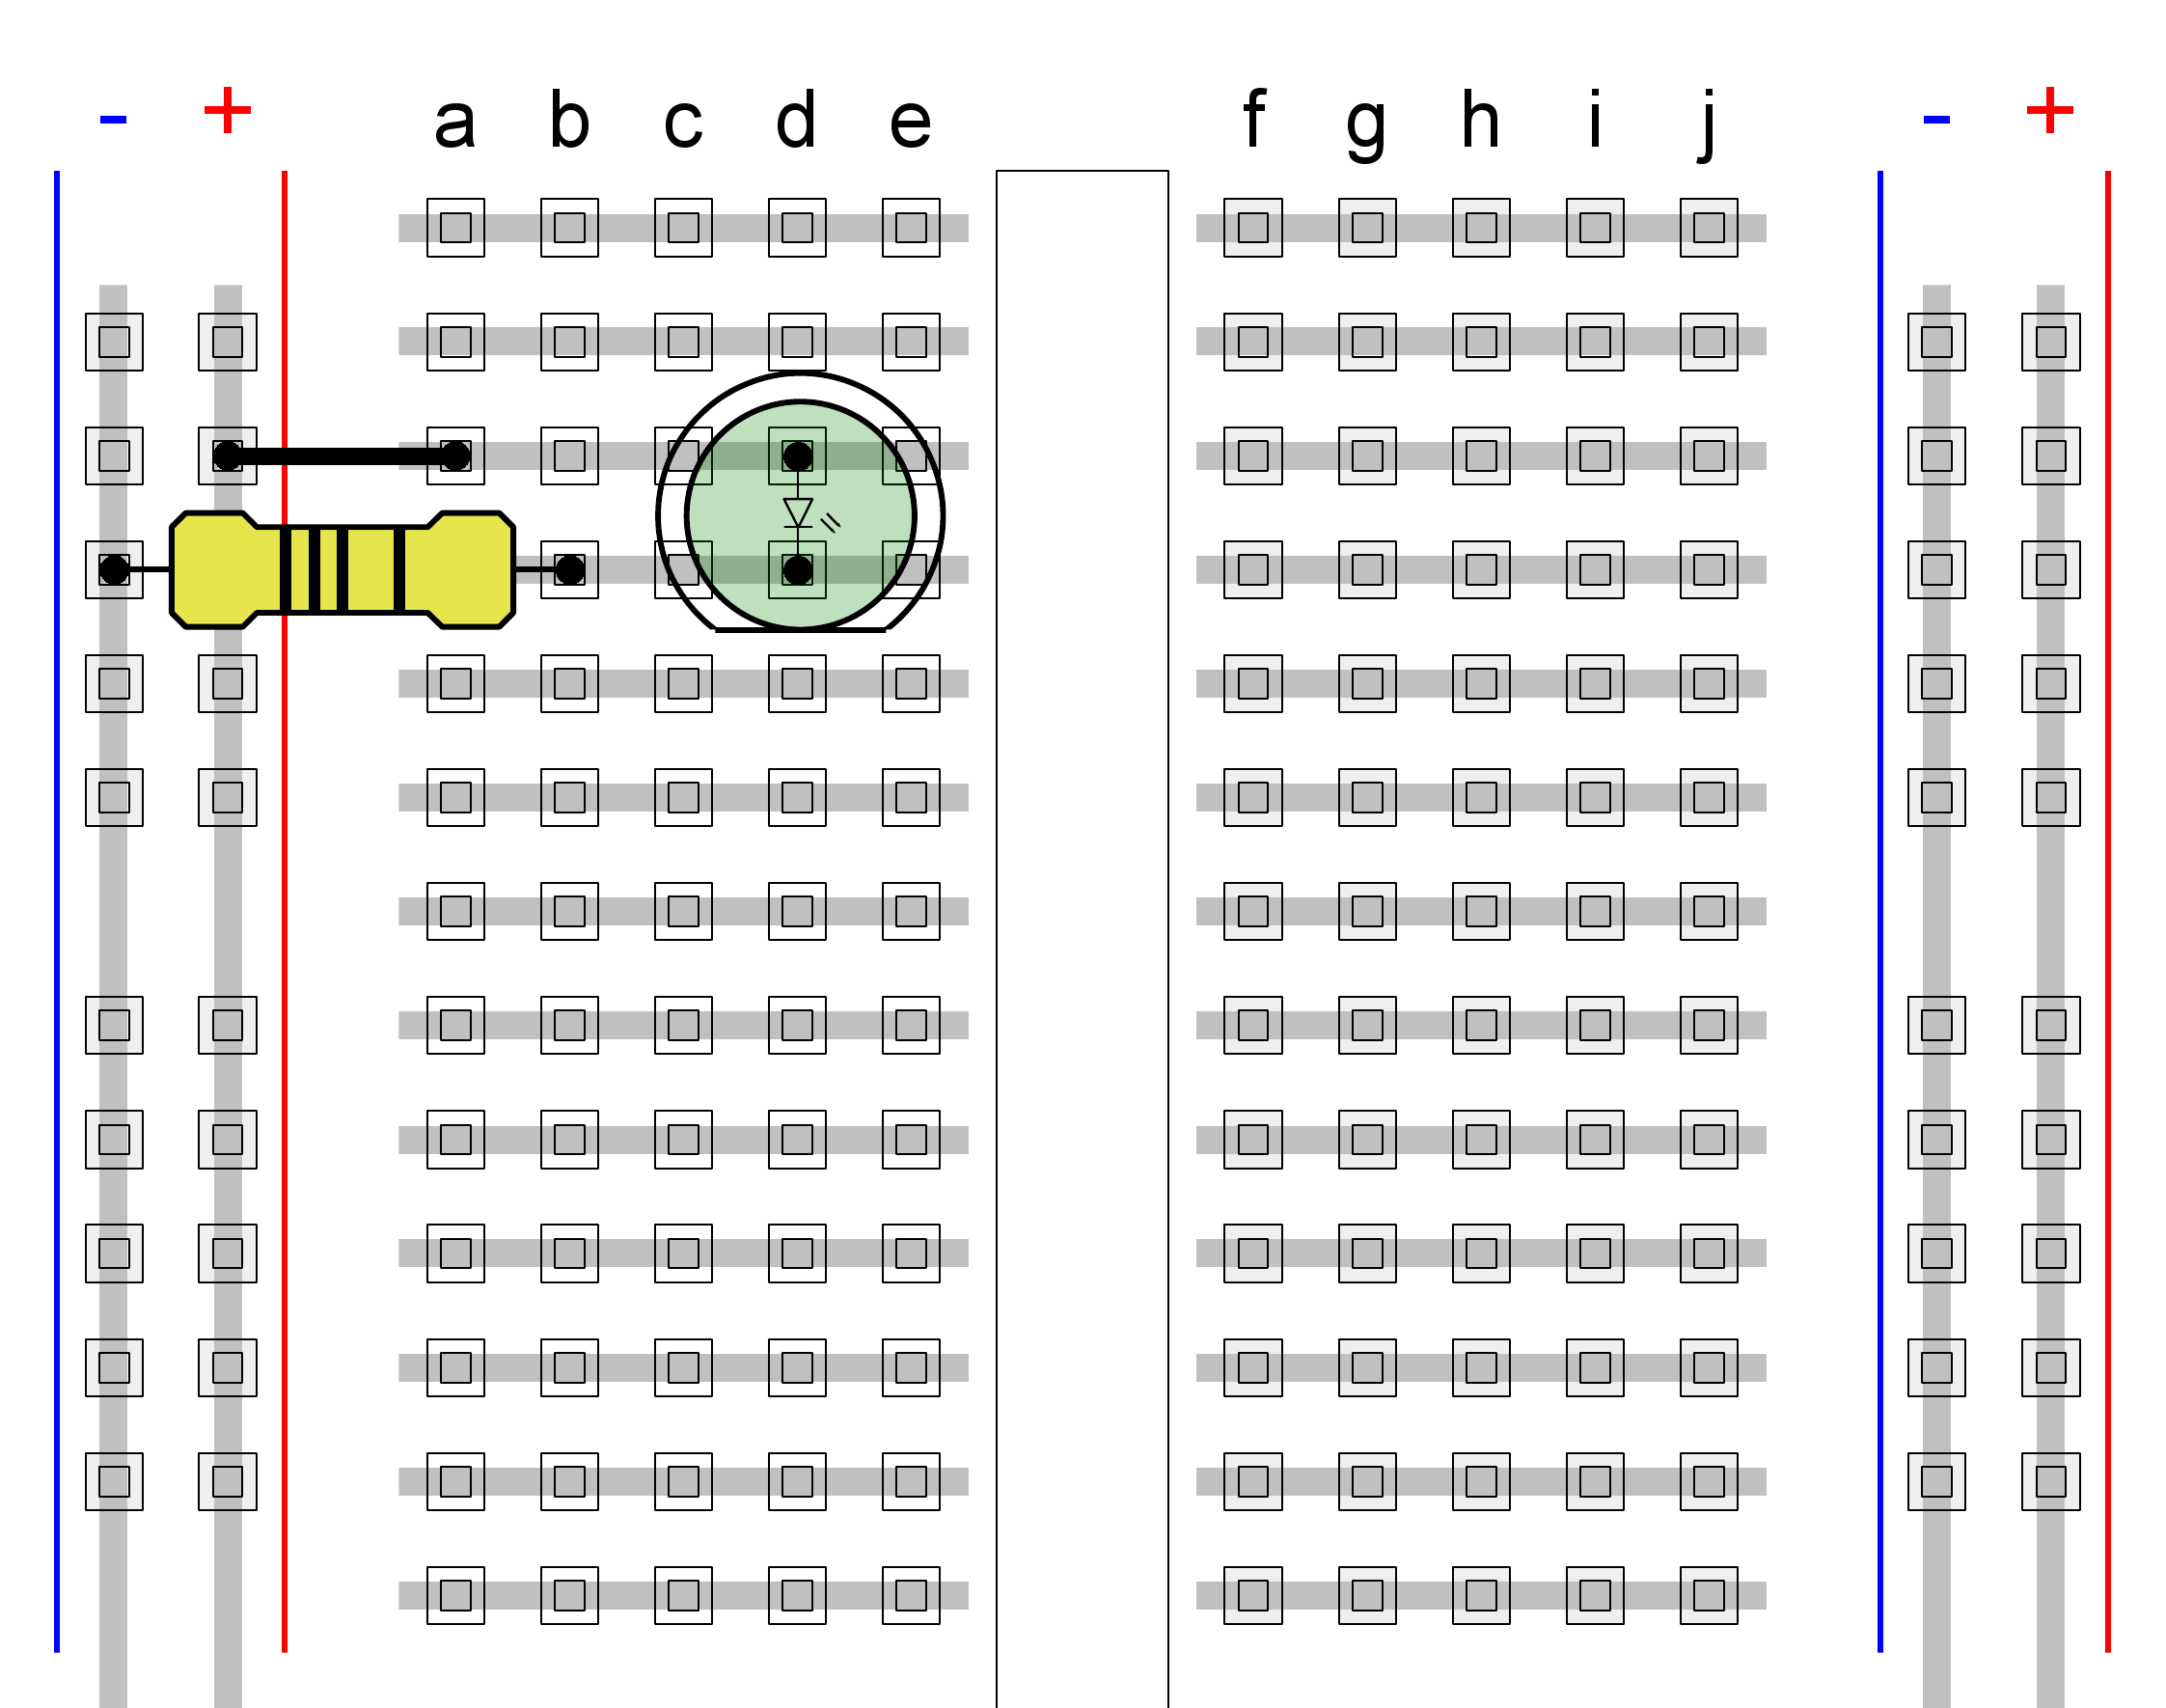
\includegraphics[width=2.4693in,height=1.9465in]{figures/ee4document-img002.png} 

{\selectlanguage{english}\sffamily\bfseries\color[rgb]{0.30980393,0.5058824,0.7411765}
Figure 10: Simple LED circuit on breadboard}

{\selectlanguage{english}\sffamily\color[rgb]{0.30980393,0.5058824,0.7411765}
However, a breadboarded circuit certainly is not going to go onto our final solar car (or any production device, for
that matter). Breadboards are handy when you are prototyping since you can easily swap out components and make changes,
but what if you want something more permanent? Something which won't fall apart given the vibrations in a car?}

{\selectlanguage{english}\sffamily\color[rgb]{0.30980393,0.5058824,0.7411765}
Enter the printed circuit board.}

\section{Technical Manual}
\hypertarget{Toc337742672}{}\subsection{What is a printed circuit board?}
\hypertarget{Toc337742673}{}{\selectlanguage{english}\sffamily\color[rgb]{0.30980393,0.5058824,0.7411765}
A \textbf{printed circuit board (PCB)} is a board on which electronic components like chips and resistors are placed and
connected.}

\subsubsection{Anatomy of a printed circuit board}
\hypertarget{Toc337742674}{} 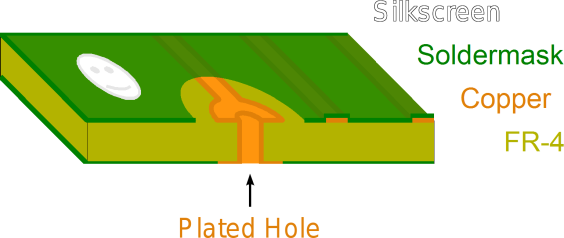
\includegraphics[width=2.5382in,height=1.0819in]{figures/ee4document-img003.png} 

{\selectlanguage{english}\sffamily\bfseries\color[rgb]{0.30980393,0.5058824,0.7411765}
Figure 10 Anatomy of a two-layer circuit board}

{\selectlanguage{english}\sffamily\color[rgb]{0.30980393,0.5058824,0.7411765}
The major parts of the board are as follows (from center upwards):}

\liststyleRTFNumxvi
\begin{itemize}
\item {\selectlanguage{english}\sffamily\color[rgb]{0.30980393,0.5058824,0.7411765}
The \textbf{substrate} makes up the bulk of the board. This is an insulating layer, and is typically made of FR-4
fiberglass laminate. Although most circuit boards appear green, the FR-4 material itself is actually yellow (more
later).}
\item {\selectlanguage{english}\sffamily\color[rgb]{0.30980393,0.5058824,0.7411765}
The \textbf{copper layer} is what makes the electrical connections. This is typically a thin layer of copper foil bonded
to the substrate, etched to the designed pattern.}

\begin{itemize}
\item {\selectlanguage{english}\sffamily\color[rgb]{0.30980393,0.5058824,0.7411765}
Features on the copper pattern also have names. A \textbf{pad} is a copper shape to which component pins are soldered,
and a \textbf{trace} is copper {\textquotedbl}wiring{\textquotedbl} connecting the pads. Sometimes, a \textbf{copper
pour} is also used to connect components - this is just an area filled with copper. Usually, a copper pour is used as a
ground.}
\end{itemize}
\item {\selectlanguage{english}\sffamily\color[rgb]{0.30980393,0.5058824,0.7411765}
The\textbf{ solder mask} is a layer of material which solder does not adhere to. This is typically applied over the
entire board minus the pads, and prevents solder from flowing onto traces.}

\begin{itemize}
\item {\selectlanguage{english}\sffamily\color[rgb]{0.30980393,0.5058824,0.7411765}
Soldermask is typically green, and is what gives circuit boards their characteristic color. However, soldermask is also
available in other colors.}
\end{itemize}
\item {\selectlanguage{english}\sffamily\color[rgb]{0.30980393,0.5058824,0.7411765}
The \textbf{silkscreen} is a layer of material for {\textquotedbl}artwork{\textquotedbl} - text and drawings on the
circuit board. This usually contains component labels (or \textbf{reference designators}), the name of the board, and
possibly component outlines.}
\end{itemize}

\bigskip

{\selectlanguage{english}\sffamily\color[rgb]{0.30980393,0.5058824,0.7411765}
Note that the board in the picture has copper on both sides, and as such, it is called a \textbf{two-layer board}.
\textbf{Vias or through-holes} are holes which pass through from one layer to another. More often than not, they are
\textbf{plated}, which makes them electrically conductive and allows them to electrically connect copper on the top and
bottom layers.}


\bigskip

{\selectlanguage{english}\sffamily\color[rgb]{0.30980393,0.5058824,0.7411765}
Boards with more layers are possible, in which case there will be \textbf{internal layers} sandwiched between insulating
substrate layers. However, cost also increases, so think really hard before deciding on a 12-layer design. Unless
you're doing a serious commercial design, 4 layers is probably the cap. CalSol usually does 2-layer boards, since we
get those sponsored by Advanced Circuits.}

{\selectlanguage{english}\sffamily\color[rgb]{0.30980393,0.5058824,0.7411765}
When there are internal layers, they typically include a dedicated \textbf{ground plane} and \textbf{power plane}, a
solid copper layer either connected to ground or power. Signals can be routed on both external and internal layers.}

\subsection{Electronic design automation (EDA)}
\hypertarget{Toc337742675}{}{\selectlanguage{english}\sffamily\color[rgb]{0.30980393,0.5058824,0.7411765}
Today, circuit diagrams and board layouts are both designed on a computer using \textbf{electronic design automation
(EDA)} or \textbf{electronic computer aided design (ECAD)} tools. This is usually a suite of tools which includes, at
the very least, schematic capture (to enter your circuit as a circuit diagram) and board layout (where you lay out the
components, traces, etc on a board) tools. Advanced features may also automatic routing, where the software will
attempt to \textbf{route} (lay out traces to connect components) for you - however, the results are only as good as the
tools.}


\bigskip

{\selectlanguage{english}\sffamily\color[rgb]{0.30980393,0.5058824,0.7411765}
Note: The category of EDA tools also include those intended for integrated circuit (IC) or chip design. These cannot be
used to lay out a circuit board.}

\clearpage
\bigskip

\subsubsection{Workflow overview}
\hypertarget{Toc337742676}{}{\selectlanguage{english}\sffamily\color[rgb]{0.30980393,0.5058824,0.7411765}
The general workflow overview for designing a circuit board is as follows:}

\liststyleRTFNumix
\begin{enumerate}
\item {\selectlanguage{english}\sffamily\color[rgb]{0.30980393,0.5058824,0.7411765}
\textbf{Idea}: You need to know what you want to do first.}
\item {\selectlanguage{english}\sffamily\color[rgb]{0.30980393,0.5058824,0.7411765}
\textbf{Circuit}: Figure out how to implement your idea using electronic parts. Prototype the circuit on a breadboard
(if possible) to ensure that it works.}
\item {\selectlanguage{english}\sffamily\color[rgb]{0.30980393,0.5058824,0.7411765}
\textbf{Schematic capture}: Enter your circuit schematic into the design suite.}
\item {\selectlanguage{english}\sffamily\color[rgb]{0.30980393,0.5058824,0.7411765}
\textbf{Board layout}: Convert your schematic into a circuit board layout, then place and route the components.}
\item {\selectlanguage{english}\sffamily\color[rgb]{0.30980393,0.5058824,0.7411765}
\textbf{Verification}: Ensure that your circuit will work as intended and is within any design constraints you may
have.}
\item {\selectlanguage{english}\sffamily\color[rgb]{0.30980393,0.5058824,0.7411765}
\textbf{Fabrication}: Generate the design files, and send them off for manufacture.}
\end{enumerate}
\subsection{Schematic capture}
\hypertarget{Toc337742677}{}{\selectlanguage{english}\sffamily\color[rgb]{0.30980393,0.5058824,0.7411765}
Schematic capture is where you entry the circuit into the design suite. Typically, this is done interactively on a
graphical representation of a schematic diagram. Basically, you insert components onto the page, and wire the
components together accordingly.}


\bigskip

{\selectlanguage{english}\sffamily\color[rgb]{0.30980393,0.5058824,0.7411765}
Once you get into a schematic editor and learn the basic controls, this should be highly straightforward and intuitive.}


\bigskip

\subsubsection{Components}
\hypertarget{Toc337742678}{}\begin{flushleft}
\tablefirsthead{}
\tablehead{}
\tabletail{}
\tablelasttail{}
\begin{supertabular}{m{2.4254599in}m{2.41916in}m{2.41916in}}
 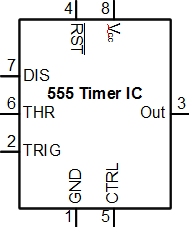
\includegraphics[width=0.9839in,height=1.1811in]{figures/ee4document-img004.png}  &
 
\includegraphics[width=0.7874in,height=0.1965in]{figures/ee4document-img005.png} 
~

 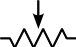
\includegraphics[width=0.7874in,height=0.4866in]{figures/ee4document-img006.png}  &
 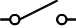
\includegraphics[width=0.7874in,height=0.289in]{figures/ee4document-img007.png} 
~

 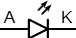
\includegraphics[width=0.7874in,height=0.3937in]{figures/ee4document-img008.png} 
~
\\
\end{supertabular}
\end{flushleft}
{\selectlanguage{english}\sffamily\color[rgb]{0.30980393,0.5058824,0.7411765}
\textbf{Figure 10 Example schematic components \& symbols}}


\bigskip

{\selectlanguage{english}\sffamily\color[rgb]{0.30980393,0.5058824,0.7411765}
A \textbf{component} is the schematic symbol for a physical electronic component. It typically has one \textbf{pin}
connection for each terminal on the device. For example, a resistor would be a component with two pins, and a 555 timer
IC would be a component with 8 pins.}

{\selectlanguage{english}\sffamily\color[rgb]{0.30980393,0.5058824,0.7411765}
Additionally, each component has an \textbf{reference designator (refdes)}. This uniquely identifies the component
within a schematic, and is usually in the format of a letter followed by a number (for example, R1, D22, and U4). The
letter indicates the type of component, and the number is just a unique identifier within that type. Common letters and
their meanings are listed below in Table 1. These are usually printed as silkscreen on the final circuit board so you
know what component does there.}

\clearpage
\bigskip

{\selectlanguage{english}\sffamily\bfseries\color[rgb]{0.30980393,0.5058824,0.7411765}
Table 4 Reference designator letters \& meanings}

\begin{flushleft}
\tablefirsthead{}
\tablehead{}
\tabletail{}
\tablelasttail{}
\begin{supertabular}{|m{0.42475984in}|m{1.9219599in}|m{0.42055985in}|m{1.9233599in}|m{0.41915986in}|m{1.9247599in}|}
\hline
{\selectlanguage{english}\sffamily\bfseries\color[rgb]{0.30980393,0.5058824,0.7411765} Letter} &
{\selectlanguage{english}\sffamily\bfseries\color[rgb]{0.30980393,0.5058824,0.7411765} Meaning} &
{\selectlanguage{english}\sffamily\bfseries\color[rgb]{0.30980393,0.5058824,0.7411765} Letter} &
{\selectlanguage{english}\sffamily\bfseries\color[rgb]{0.30980393,0.5058824,0.7411765} Meaning} &
{\selectlanguage{english}\sffamily\bfseries\color[rgb]{0.30980393,0.5058824,0.7411765} Letter} &
{\selectlanguage{english}\sffamily\bfseries\color[rgb]{0.30980393,0.5058824,0.7411765} Meaning}\\\hline
{\selectlanguage{english}\sffamily\bfseries\color[rgb]{0.30980393,0.5058824,0.7411765} C} &
{\selectlanguage{english}\sffamily\color[rgb]{0.30980393,0.5058824,0.7411765} Capacitors} &
{\selectlanguage{english}\sffamily\bfseries\color[rgb]{0.30980393,0.5058824,0.7411765} L} &
{\selectlanguage{english}\sffamily\color[rgb]{0.30980393,0.5058824,0.7411765} Inductors} &
{\selectlanguage{english}\sffamily\bfseries\color[rgb]{0.30980393,0.5058824,0.7411765} TP} &
{\selectlanguage{english}\sffamily\color[rgb]{0.30980393,0.5058824,0.7411765} Test points}\\\hline
{\selectlanguage{english}\sffamily\bfseries\color[rgb]{0.30980393,0.5058824,0.7411765} D} &
{\selectlanguage{english}\sffamily\color[rgb]{0.30980393,0.5058824,0.7411765} Discrete diodes, including LEDs} &
{\selectlanguage{english}\sffamily\bfseries\color[rgb]{0.30980393,0.5058824,0.7411765} Q} &
{\selectlanguage{english}\sffamily\color[rgb]{0.30980393,0.5058824,0.7411765} Transistors} &
{\selectlanguage{english}\sffamily\bfseries\color[rgb]{0.30980393,0.5058824,0.7411765} U} &
{\selectlanguage{english}\sffamily\color[rgb]{0.30980393,0.5058824,0.7411765} Integrated circuits and misc.}\\\hline
{\selectlanguage{english}\sffamily\bfseries\color[rgb]{0.30980393,0.5058824,0.7411765} F} &
{\selectlanguage{english}\sffamily\color[rgb]{0.30980393,0.5058824,0.7411765} Fuses} &
{\selectlanguage{english}\sffamily\bfseries\color[rgb]{0.30980393,0.5058824,0.7411765} R} &
{\selectlanguage{english}\sffamily\color[rgb]{0.30980393,0.5058824,0.7411765} Resistors} &
{\selectlanguage{english}\sffamily\bfseries\color[rgb]{0.30980393,0.5058824,0.7411765} X} &
{\selectlanguage{english}\sffamily\color[rgb]{0.30980393,0.5058824,0.7411765} Crystals}\\\hline
{\selectlanguage{english}\sffamily\bfseries\color[rgb]{0.30980393,0.5058824,0.7411765} J} &
{\selectlanguage{english}\sffamily\color[rgb]{0.30980393,0.5058824,0.7411765} Connectors} &
{\selectlanguage{english}\sffamily\color[rgb]{0.30980393,0.5058824,0.7411765} \textbf{S / SW}} &
{\selectlanguage{english}\sffamily\color[rgb]{0.30980393,0.5058824,0.7411765} Switches} &
~
 &
~
\\\hline
\end{supertabular}
\end{flushleft}

\bigskip

{\selectlanguage{english}\sffamily\color[rgb]{0.30980393,0.5058824,0.7411765}
In most programs, picking a component also includes picking its \textbf{package} or \textbf{pattern}, which is the form
a component comes in. For example, a resistor can be in several different sizes (like 1/4 watt, 1/2 watt or even
surface-mount 0603 - each requiring different copper and drill patterns), and the package determines which one it is.
For integrated circuits, the same chip often comes in many different packages, possibly including a mix of through-hole
and surface-mount. Common device packages are listed in Table 2. Google and Wikipedia should have many pictures.}


\bigskip

{\selectlanguage{english}\sffamily\color[rgb]{0.30980393,0.5058824,0.7411765}
\textbf{Through-hole} components are designed to have their pins inserted into a plated hole. Then, the hole is filled
with solder which electrically and mechanically connects the component to the board.}

{\selectlanguage{english}\sffamily\color[rgb]{0.30980393,0.5058824,0.7411765}
\textbf{Surface-mount} components don't have {\textquotedbl}pins{\textquotedbl} in the traditional sense. They are
designed to be placed on top of the board with their terminals soldered to a pad. These components are typically much
smaller than their through-hole counterparts - and may be more difficult to manually solder. }

\begin{flushleft}
\tablefirsthead{}
\tablehead{}
\tabletail{}
\tablelasttail{}
\begin{supertabular}{m{3.7275598in}m{3.6150599in}}
 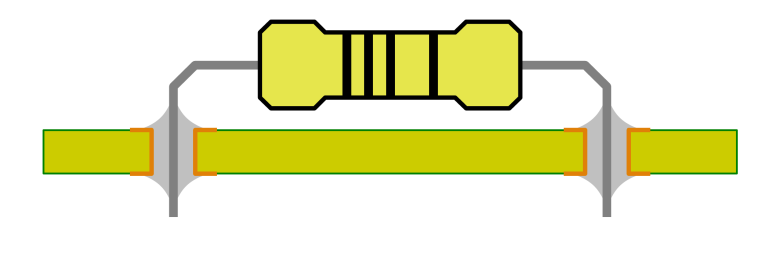
\includegraphics[width=3.5457in,height=1.1819in]{figures/ee4document-img009.png} 
{\selectlanguage{english}\sffamily\bfseries\color[rgb]{0.30980393,0.5058824,0.7411765} Figure 10 A through-hole
resistor} &
 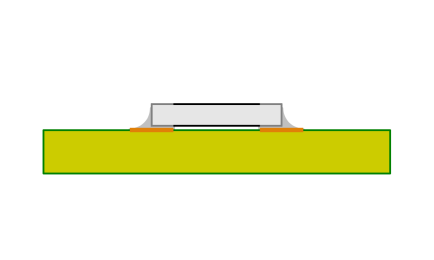
\includegraphics[width=1.9728in,height=1.1819in]{figures/ee4document-img010.png} 
{\selectlanguage{english}\sffamily\bfseries\color[rgb]{0.30980393,0.5058824,0.7411765} Figure 10 A surface-mount
resistor}\\
\end{supertabular}
\end{flushleft}
{\selectlanguage{english}\sffamily\bfseries\color[rgb]{0.30980393,0.5058824,0.7411765}
Table 4 Non-exhaustive listing of common device packages as seen by CalSol / hobbyists -- industry goes much smaller}

\begin{flushleft}
\tablefirsthead{}
\tablehead{}
\tabletail{}
\tablelasttail{}
\begin{supertabular}{|m{2.4254599in}|m{2.4226599in}|m{2.4226599in}|}
\hline
{\selectlanguage{english}\sffamily\bfseries\color[rgb]{0.30980393,0.5058824,0.7411765} Device} &
{\selectlanguage{english}\sffamily\color[rgb]{0.30980393,0.5058824,0.7411765} \textbf{Common through-hole packages}} &
{\selectlanguage{english}\sffamily\color[rgb]{0.30980393,0.5058824,0.7411765} \textbf{Common surface-mount
packages}}\\\hline
{\selectlanguage{english}\sffamily\bfseries\color[rgb]{0.30980393,0.5058824,0.7411765} Discrete capacitors} &
{\selectlanguage{english}\sffamily\color[rgb]{0.30980393,0.5058824,0.7411765} various} &
{\selectlanguage{english}\sffamily\color[rgb]{0.30980393,0.5058824,0.7411765} 0402, 0603, 0805, 1206}

{\selectlanguage{english}\sffamily\color[rgb]{0.30980393,0.5058824,0.7411765} (for small capacitances)}\\\hline
{\selectlanguage{english}\sffamily\bfseries\color[rgb]{0.30980393,0.5058824,0.7411765} Discrete resistors} &
{\selectlanguage{english}\sffamily\color[rgb]{0.30980393,0.5058824,0.7411765} 1/4 watt, 1/8 watt} &
{\selectlanguage{english}\sffamily\color[rgb]{0.30980393,0.5058824,0.7411765} 0402, 0603, 0805, 1206}\\\hline
{\selectlanguage{english}\sffamily\bfseries\color[rgb]{0.30980393,0.5058824,0.7411765} Inductors} &
{\selectlanguage{english}\sffamily\color[rgb]{0.30980393,0.5058824,0.7411765} various} &
{\selectlanguage{english}\sffamily\color[rgb]{0.30980393,0.5058824,0.7411765} various}\\\hline
{\selectlanguage{english}\sffamily\bfseries\color[rgb]{0.30980393,0.5058824,0.7411765} LEDs} &
{\selectlanguage{english}\sffamily\color[rgb]{0.30980393,0.5058824,0.7411765} T 1{\textthreequarters} (5mm), T 1 (3mm)}
&
{\selectlanguage{english}\sffamily\color[rgb]{0.30980393,0.5058824,0.7411765} 0603, 0805, 1206}\\\hline
{\selectlanguage{english}\sffamily\bfseries\color[rgb]{0.30980393,0.5058824,0.7411765} Diodes} &
{\selectlanguage{english}\sffamily\color[rgb]{0.30980393,0.5058824,0.7411765} various} &
{\selectlanguage{english}\sffamily\color[rgb]{0.30980393,0.5058824,0.7411765} various}\\\hline
{\selectlanguage{english}\sffamily\bfseries\color[rgb]{0.30980393,0.5058824,0.7411765} Transistors} &
{\selectlanguage{english}\sffamily\color[rgb]{0.30980393,0.5058824,0.7411765} TO-92, TO-220} &
{\selectlanguage{english}\sffamily\color[rgb]{0.30980393,0.5058824,0.7411765} SOT-23, SOT-89}\\\hline
{\selectlanguage{english}\sffamily\bfseries\color[rgb]{0.30980393,0.5058824,0.7411765} Integrated circuits} &
{\selectlanguage{english}\sffamily\color[rgb]{0.30980393,0.5058824,0.7411765} DIP-x}

{\selectlanguage{english}\sffamily\color[rgb]{0.30980393,0.5058824,0.7411765} (where x is the number of pins)} &
{\selectlanguage{english}\sffamily\color[rgb]{0.30980393,0.5058824,0.7411765} SOIC-x, SSOP-x, TQFP-x, QFN-x}

{\selectlanguage{english}\sffamily\color[rgb]{0.30980393,0.5058824,0.7411765} (where x is the number of pins)}\\\hline
\end{supertabular}
\end{flushleft}

\bigskip

\clearpage
\bigskip

\subsubsection{Basic concepts}
\hypertarget{Toc337742679}{}{\selectlanguage{english}\sffamily\color[rgb]{0.30980393,0.5058824,0.7411765}
Schematics can be organized into \textbf{pages} - each corresponding to a physical sheet of paper which contains part of
a circuit.}

{\selectlanguage{english}\sffamily\color[rgb]{0.30980393,0.5058824,0.7411765}
Then, there is the issue of connectivity, which is represented by \textbf{nets}. These basically state what pins on what
components are connected together. You can think of a net as a wire - all pins which are part of a net are electrically
connected together}

{\selectlanguage{english}\sffamily\color[rgb]{0.30980393,0.5058824,0.7411765}
On some design suites, nets can be named. However, whenever you create a new wire, they are typically given some generic
name, like {\textquotedbl}Net 42.{\textquotedbl}}

{\selectlanguage{english}\sffamily\color[rgb]{0.30980393,0.5058824,0.7411765}
Individual wires on a schematic can also be combined into a \textbf{bus}. A bus is essentially a bundle of wires, and
individual wires can branch off of it. Busses are used to keep a schematic clean - instead of trying to route 10
different wires, you can have just one thick wire with individual wires branching off at the source and destination.}


\bigskip

{\selectlanguage{english}\sffamily\color[rgb]{0.30980393,0.5058824,0.7411765}
To simplify wiring, there are also \textbf{tunnels} - all wires entering a tunnel with the same name are connected. This
allows you to connect components on different pages, or even connect components on the same page without needing a
wire. Good use of tunnels can keep a schematic clean.}

{\selectlanguage{english}\sffamily\color[rgb]{0.30980393,0.5058824,0.7411765}
The implementation of this feature varies by software. Sometimes, you may need to add an actual tunnel object which can
be named. On others, this is simply implemented by adding wires to a common net.}

{\selectlanguage{english}\sffamily\color[rgb]{0.30980393,0.5058824,0.7411765}
Finally, there are the power supplies - usually the symbols 
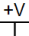
\includegraphics[width=0.1291in,height=0.1618in]{figures/ee4document-img011.png}  for a positive voltage source and 
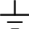
\includegraphics[width=0.1291in,height=0.1291in]{figures/ee4document-img012.png}  for ground (0v). Like tunnels, these are all
implicitly connected to the same net.}


\bigskip

\subsubsection{Good practices}
\hypertarget{Toc337742680}{}{\selectlanguage{english}\sffamily\color[rgb]{0.30980393,0.5058824,0.7411765}
Following good practices helps ensure readability and correctness.}

\liststyleRTFNumxiv
\begin{itemize}
\item {\selectlanguage{english}\sffamily\color[rgb]{0.30980393,0.5058824,0.7411765}
Convention says that a circuit should {\textquotedbl}flow{\textquotedbl} from left to right - inputs on the left and
outputs on the right.}
\item {\selectlanguage{english}\sffamily\color[rgb]{0.30980393,0.5058824,0.7411765}
Modularize your schematic - keep related parts together. Make use of different pages if your schematic is large enough.}
\item {\selectlanguage{english}\sffamily\color[rgb]{0.30980393,0.5058824,0.7411765}
\textbf{Keep your circuits legible and clean}. I cannot stress how important this is. Messiness can conceal bugs - stuff
you might not notice until after you receive and assemble your boards, only to figure out it does not work and you have
a very expensive brick.}

\begin{itemize}
\item {\selectlanguage{english}\sffamily\color[rgb]{0.30980393,0.5058824,0.7411765}
Crisscrossing wires may impair legibility. Although the rule is that crossed wires are only connected if there is a dot
present, it may not be obvious at a quick glance.}
\item {\selectlanguage{english}\sffamily\color[rgb]{0.30980393,0.5058824,0.7411765}
Consider labeling portions of your schematic with a brief description of what it does. }
\item {\selectlanguage{english}\sffamily\color[rgb]{0.30980393,0.5058824,0.7411765}
Avoid having wires that go nowhere.}
\item {\selectlanguage{english}\sffamily\color[rgb]{0.30980393,0.5058824,0.7411765}
Consider using tunnels. This can also help modularize your schematic as well, eliminating the need for wires running
across the schematic. When using tunnels, make sure that they are named intuitively. A tunnel named ``Net 42'' is not
helpful; while a tunnel named ``SPI\_MISO'' is clear in what it does.}
\end{itemize}
\item {\selectlanguage{english}\sffamily\color[rgb]{0.30980393,0.5058824,0.7411765}
Aesthetics: Schematics are not art, but it is usually a good idea to make them look nice.}

\begin{itemize}
\item {\selectlanguage{english}\sffamily\color[rgb]{0.30980393,0.5058824,0.7411765}
For example, if you have a row of LEDs, place them such that they are aligned and evenly spaced.}
\item {\selectlanguage{english}\sffamily\color[rgb]{0.30980393,0.5058824,0.7411765}
Consistency is another point under aesthetics. If you decide to do something one way, stick with it. For example, if you
put the current limiting resistors on the low side of a LED, do that across your schematic - don't mix low-side and
high-side resistors.}
\item {\selectlanguage{english}\sffamily\color[rgb]{0.30980393,0.5058824,0.7411765}
However, this is usually a matter of personal taste. Use your best judgment.}
\end{itemize}
\end{itemize}
\subsection{Board layout}
\hypertarget{Toc337742681}{}{\selectlanguage{english}\sffamily\color[rgb]{0.30980393,0.5058824,0.7411765}
The board layout is where you actually lay out the circuit board design. Typically, this is done in a different program
than the schematic editor. However, you should be able to convert your schematic into a board design. Connectivity data
and components will be forwarded to the board design program, but that's about it - current software cannot
automatically create a full circuit board layout based off a schematic.}

\subsubsection{Basic concepts}
\hypertarget{Toc337742682}{}{\selectlanguage{english}\sffamily\color[rgb]{0.30980393,0.5058824,0.7411765}
Similar to schematic capture, you again have components and wires. However, now, you are physically locating the
component \textbf{footprint or pattern} - the pads which the components will be soldered to - on a board. Be careful
not to make your design impossible to assemble - in particular, components should not overlap. Often, components have
an outline on the silkscreen layer, and this should help prevent conflicts.}

{\selectlanguage{english}\sffamily\color[rgb]{0.30980393,0.5058824,0.7411765}
You can move components around the board, and on double-sided boards, you can also flip components to the back side.
Flipping is recommended only for surface-mount components, and usually only when you cannot fit all the components on
one side. Double-sided boards increase the complexity (and thus cost) of reflow soldering,}

\begin{flushleft}
\tablefirsthead{}
\tablehead{}
\tabletail{}
\tablelasttail{}
\begin{supertabular}{m{3.7275598in}m{3.6150599in}}
 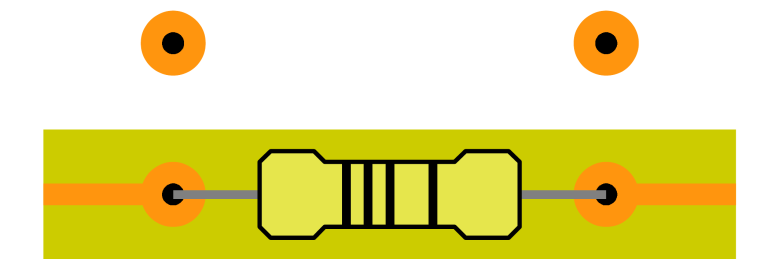
\includegraphics[width=3.5409in,height=1.1772in]{figures/ee4document-img013.png} 
{\selectlanguage{english}\sffamily\bfseries\color[rgb]{0.30980393,0.5058824,0.7411765} Figure 10 Through-hole resistor:
pattern (top), actual layout (bottom)} &
 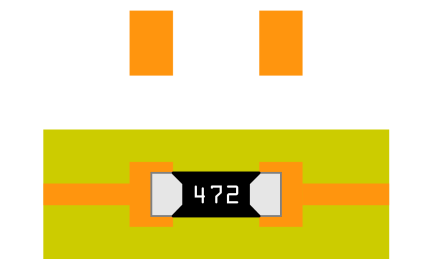
\includegraphics[width=1.9681in,height=1.1772in]{figures/ee4document-img014.png} 
{\selectlanguage{english}\sffamily\bfseries\color[rgb]{0.30980393,0.5058824,0.7411765} Figure 10 Surface-mount resistor:
pattern (top), actual layout (bottom)}\\
\end{supertabular}
\end{flushleft}
{\selectlanguage{english}\sffamily\color[rgb]{0.30980393,0.5058824,0.7411765}
You will also \textbf{route} your board here - lay out the traces that will connect the pads on the components. You can
route connections on any copper layer (and connect the different layers using vias), but all traces on a single layer
forms a solid piece of copper. Therefore, if you have intersecting copper traces on the same layer, they are
electrically connected. If you do not want that to happen, you must route the paths on different copper layers.}


\bigskip

{\selectlanguage{english}\sffamily\color[rgb]{0.30980393,0.5058824,0.7411765}
When connectivity data is forwarded from a schematic, a \textbf{rats nest} (consisting of individual \textbf{ratlines})
is used to indicate unrouted connections. Once all these disappear, you have routed your entire board.}


\bigskip

{\selectlanguage{english}\sffamily\color[rgb]{0.30980393,0.5058824,0.7411765}
Finally, you will need to define your \textbf{board outline}, which indicates the physical edges of the board.}

\subsubsection{Design rules}
\hypertarget{Toc337742683}{}{\selectlanguage{english}\sffamily\color[rgb]{0.30980393,0.5058824,0.7411765}
Unfortunately, there are limits to what a board house can do - and these manufacturing capabilities are captured in the
design rules. A quick listing is in Table 3.}


\bigskip

{\selectlanguage{english}\sffamily\bfseries\color[rgb]{0.30980393,0.5058824,0.7411765}
Table 4 Common design rules, their descriptions, and common values}

\begin{flushleft}
\tablefirsthead{}
\tablehead{}
\tabletail{}
\tablelasttail{}
\begin{supertabular}{|m{1.4247599in}|m{4.42126in}|m{1.4247599in}|}
\hline
{\selectlanguage{english}\sffamily\bfseries\color[rgb]{0.30980393,0.5058824,0.7411765} Rule} &
{\selectlanguage{english}\sffamily\bfseries\color[rgb]{0.30980393,0.5058824,0.7411765} Description} &
{\selectlanguage{english}\sffamily\bfseries\color[rgb]{0.30980393,0.5058824,0.7411765} Common values}\\\hline
{\selectlanguage{english}\sffamily\bfseries\color[rgb]{0.30980393,0.5058824,0.7411765} Minimum trace width} &
{\selectlanguage{english}\sffamily\color[rgb]{0.30980393,0.5058824,0.7411765} The minimum width of any copper shape} &
{\selectlanguage{english}\sffamily\color[rgb]{0.30980393,0.5058824,0.7411765} 6 mil, 8 mil}\\\hline
{\selectlanguage{english}\sffamily\bfseries\color[rgb]{0.30980393,0.5058824,0.7411765} Minimum trace spacing} &
{\selectlanguage{english}\sffamily\color[rgb]{0.30980393,0.5058824,0.7411765} The minimum spacing between two
non-connected copper shapes} &
{\selectlanguage{english}\sffamily\color[rgb]{0.30980393,0.5058824,0.7411765} 6 mil, 8 mil}\\\hline
{\selectlanguage{english}\sffamily\bfseries\color[rgb]{0.30980393,0.5058824,0.7411765} Minimum drill size} &
{\selectlanguage{english}\sffamily\color[rgb]{0.30980393,0.5058824,0.7411765} The minimum size of any via or hole} &
{\selectlanguage{english}\sffamily\color[rgb]{0.30980393,0.5058824,0.7411765} 13 mil, 20 mil}\\\hline
{\selectlanguage{english}\sffamily\bfseries\color[rgb]{0.30980393,0.5058824,0.7411765} Maximum drill size} &
{\selectlanguage{english}\sffamily\color[rgb]{0.30980393,0.5058824,0.7411765} The maximum size of any via or hole} &
{\selectlanguage{english}\sffamily\color[rgb]{0.30980393,0.5058824,0.7411765} big}\\\hline
{\selectlanguage{english}\sffamily\bfseries\color[rgb]{0.30980393,0.5058824,0.7411765} Annular ring} &
{\selectlanguage{english}\sffamily\color[rgb]{0.30980393,0.5058824,0.7411765} The minimum copper ring width around any
plated via or hole} &
{\selectlanguage{english}\sffamily\color[rgb]{0.30980393,0.5058824,0.7411765} same as trace width}\\\hline
\end{supertabular}
\end{flushleft}
{\selectlanguage{english}\sffamily\color[rgb]{0.30980393,0.5058824,0.7411765}
* 1 mil = 1/1000 in = 0.0254 mm}


\bigskip

{\selectlanguage{english}\sffamily\color[rgb]{0.30980393,0.5058824,0.7411765}
So, no, you can't make 22nm circuits on a circuit board.}

\subsubsection{Practical considerations}
\hypertarget{Toc337742684}{}{\selectlanguage{english}\sffamily\color[rgb]{0.30980393,0.5058824,0.7411765}
Although you can design for the limits, doing so may affect reliability. In general, you want to design for loose
tolerances, keeping trace sizes and spacings wider than the minimum.}

{\selectlanguage{english}\sffamily\color[rgb]{0.30980393,0.5058824,0.7411765}
Additionally, traces are made of copper, which is \textit{not} a perfect conductor. They have resistance, which causes
voltage drop and heat. A wider trace or a shorter trace will help reduce resistance and voltage drop. In particular,
power traces are generally wider than signal traces.}

{\selectlanguage{english}\sffamily\color[rgb]{0.30980393,0.5058824,0.7411765}
There are online tools which can calculate the minimum trace width given the current going through it and maximum
temperature rise.}

\subsubsection{Good practices}
\hypertarget{Toc337742685}{}\liststyleRTFNumvii
\begin{itemize}
\item {\selectlanguage{english}\sffamily\color[rgb]{0.30980393,0.5058824,0.7411765}
Do not design for the minimums unless you absolutely have to. Doing so can increase both failure rates and cost.}
\item {\selectlanguage{english}\sffamily\color[rgb]{0.30980393,0.5058824,0.7411765}
Plan, plan, plan. Proper component placement can make routing prettier and easier.}
\item {\selectlanguage{english}\sffamily\color[rgb]{0.30980393,0.5058824,0.7411765}
Place components such that they are aligned to the grid.}
\item {\selectlanguage{english}\sffamily\color[rgb]{0.30980393,0.5058824,0.7411765}
Route such that the traces are aligned to the grid. For this, you may want to select a finer grid than the component
placement grid.}
\item {\selectlanguage{english}\sffamily\color[rgb]{0.30980393,0.5058824,0.7411765}
Avoid overlapping components unless you really, really, REALLY, know what you are doing. This generally makes assembly
and rework difficult.}

\begin{itemize}
\item {\selectlanguage{english}\sffamily\color[rgb]{0.30980393,0.5058824,0.7411765}
You MUST NOT overlap surface-mount components - this can make the board impossible to solder.}
\end{itemize}
\item {\selectlanguage{english}\sffamily\color[rgb]{0.30980393,0.5058824,0.7411765}
\ Ensure the board is easy to assemble and rework.}

\begin{itemize}
\item {\selectlanguage{english}\sffamily\color[rgb]{0.30980393,0.5058824,0.7411765}
For example, if you have a short component surrounded by tall components, you will have one heck of a time trying to
replace that component should it be defective.}
\end{itemize}
\item {\selectlanguage{english}\sffamily\color[rgb]{0.30980393,0.5058824,0.7411765}
If space permits, consider adding a ground plane and a power plane. On 4-layer boards, the two inner layers usually are
a power plane and a ground plane.}
\item {\selectlanguage{english}\sffamily\color[rgb]{0.30980393,0.5058824,0.7411765}
All traces should be angled at some multiple of 45{\textdegree}.}
\item {\selectlanguage{english}\sffamily\color[rgb]{0.30980393,0.5058824,0.7411765}
Route boards such that all angles between traces are at 45{\textdegree}.}

\begin{itemize}
\item {\selectlanguage{english}\sffamily\color[rgb]{0.30980393,0.5058824,0.7411765}
90 degree angles are permitted, but discouraged. Sharp angles may cause interference and distortion on high speed
signals.}
\end{itemize}
\item {\selectlanguage{english}\sffamily\color[rgb]{0.30980393,0.5058824,0.7411765}
Consistency and patterns. Your board should look aesthetically pleasing.}
\item {\selectlanguage{english}\sffamily\color[rgb]{0.30980393,0.5058824,0.7411765}
For high frequency circuits (well into the MHz range), poor layout can result in coupling between adjacent signals,
which can cause corruption and data loss.}

\begin{itemize}
\item {\selectlanguage{english}\sffamily\color[rgb]{0.30980393,0.5058824,0.7411765}
In particular, signals laid out in parallel can be subject to \textbf{crosstalk}, where one signal affects another line.
The specific details are outside the scope of this document.}
\end{itemize}
\end{itemize}
\subsection{Fabrication}
\hypertarget{Toc337742686}{}{\selectlanguage{english}\sffamily\color[rgb]{0.30980393,0.5058824,0.7411765}
So you've laid out your board. Now what?}

\subsubsection{Verification \& design rule checking (DRC)}
\hypertarget{Toc337742687}{}{\selectlanguage{english}\sffamily\color[rgb]{0.30980393,0.5058824,0.7411765}
Before you put down money to have your board fabricated, you want to make sure it works.}

{\selectlanguage{english}\sffamily\color[rgb]{0.30980393,0.5058824,0.7411765}
Your design software will probably have tools to \textbf{check net connectivity} - verify that everything that you want
connected is indeed connected.}

{\selectlanguage{english}\sffamily\color[rgb]{0.30980393,0.5058824,0.7411765}
Your design software will probably also have a \textbf{design rules checker (DRC)} - run this to make sure that the
board layout meets the design rules. However, your board house will also run their own DRC before they begin
fabrication}

{\selectlanguage{english}\sffamily\color[rgb]{0.30980393,0.5058824,0.7411765}
Also consider getting your board \textbf{design reviewed} by another person (or send out a request to the entire team!)}

\subsubsection{Gerbers}
\hypertarget{Toc337742688}{}{\selectlanguage{english}\sffamily\color[rgb]{0.30980393,0.5058824,0.7411765}
Gerbers ... as in baby food? Not quite.}

{\selectlanguage{english}\sffamily\color[rgb]{0.30980393,0.5058824,0.7411765}
Gerbers (RS-274X) are the standard file format for PCB manufacturing data, and all board design software should be able
to export in this format.}

{\selectlanguage{english}\sffamily\color[rgb]{0.30980393,0.5058824,0.7411765}
Each Gerber file defines a 2d vector image, and you will have one Gerber file for each board layer. The common layers
are listed in Table 4.}

{\selectlanguage{english}\sffamily\color[rgb]{0.30980393,0.5058824,0.7411765}
In addition to the Gerbers, you also need a file to define the drilled holes in your board. This is typically
accomplished in a NC Drill (or Excellon format) file.}


\bigskip

{\selectlanguage{english}\sffamily\bfseries\color[rgb]{0.30980393,0.5058824,0.7411765}
Table 4 Fabrication data - note that extensions do vary, and additional fabrication data exists - this is the bare
minimum}

\begin{flushleft}
\tablefirsthead{}
\tablehead{}
\tabletail{}
\tablelasttail{}
\begin{supertabular}{|m{0.9247598in}|m{6.42476in}|}
\hline
{\selectlanguage{english}\sffamily\bfseries\color[rgb]{0.30980393,0.5058824,0.7411765} Extension} &
{\selectlanguage{english}\sffamily\bfseries\color[rgb]{0.30980393,0.5058824,0.7411765} Function}\\\hline
{\selectlanguage{english}\sffamily\bfseries\color[rgb]{0.30980393,0.5058824,0.7411765} .gbr} &
{\selectlanguage{english}\sffamily\color[rgb]{0.30980393,0.5058824,0.7411765} Generic Gerber file}\\\hline
{\selectlanguage{english}\sffamily\bfseries\color[rgb]{0.30980393,0.5058824,0.7411765} .gtl} &
{\selectlanguage{english}\sffamily\color[rgb]{0.30980393,0.5058824,0.7411765} Top copper layer Gerber}\\\hline
{\selectlanguage{english}\sffamily\bfseries\color[rgb]{0.30980393,0.5058824,0.7411765} .gbl} &
{\selectlanguage{english}\sffamily\color[rgb]{0.30980393,0.5058824,0.7411765} Bottom copper layer Gerber}\\\hline
{\selectlanguage{english}\sffamily\bfseries\color[rgb]{0.30980393,0.5058824,0.7411765} .gto} &
{\selectlanguage{english}\sffamily\color[rgb]{0.30980393,0.5058824,0.7411765} Top silkscreen layer Gerber}\\\hline
{\selectlanguage{english}\sffamily\bfseries\color[rgb]{0.30980393,0.5058824,0.7411765} .gbo} &
{\selectlanguage{english}\sffamily\color[rgb]{0.30980393,0.5058824,0.7411765} Bottom silkscreen layer Gerber}\\\hline
{\selectlanguage{english}\sffamily\color[rgb]{0.30980393,0.5058824,0.7411765} \textbf{.gts}} &
{\selectlanguage{english}\sffamily\color[rgb]{0.30980393,0.5058824,0.7411765} Top soldermask layer Gerber}\\\hline
{\selectlanguage{english}\sffamily\bfseries\color[rgb]{0.30980393,0.5058824,0.7411765} .gbs} &
{\selectlanguage{english}\sffamily\color[rgb]{0.30980393,0.5058824,0.7411765} Bottom soldermask layer Gerber}\\\hline
{\selectlanguage{english}\sffamily\bfseries\color[rgb]{0.30980393,0.5058824,0.7411765} .drl, .txt} &
{\selectlanguage{english}\sffamily\color[rgb]{0.30980393,0.5058824,0.7411765} NC Drill file}\\\hline
{\selectlanguage{english}\sffamily\bfseries\color[rgb]{0.30980393,0.5058824,0.7411765} .oln, .outline} &
{\selectlanguage{english}\sffamily\color[rgb]{0.30980393,0.5058824,0.7411765} Board outline Gerber}\\\hline
\end{supertabular}
\end{flushleft}
{\selectlanguage{english}\sffamily\color[rgb]{0.30980393,0.5058824,0.7411765}
Once you have generated all these files from your design, you send these to the manufacturer. Once they have ensured
that your board meets their design rules, they will produce the board and ship it to you.}

\subsection{Assembly}
\hypertarget{Toc337742689}{}{\selectlanguage{english}\sffamily\color[rgb]{0.30980393,0.5058824,0.7411765}
Once you get your boards in the mail, you can assemble them by soldering components onto the board. However, that is a
subject for another lab on another day.}

\subsection{Advanced: Component creation}
\hypertarget{Toc337742690}{}{\selectlanguage{english}\sffamily\color[rgb]{0.30980393,0.5058824,0.7411765}
Most board design suites come with a \textbf{library} of predefined components. These include schematic symbols and
patterns for the most common components and packages.}

{\selectlanguage{english}\sffamily\color[rgb]{0.30980393,0.5058824,0.7411765}
However, every once in a while, you may want to use a component that is not already available. To do so, you will have
to create your own schematic symbol and pattern.}

\subsubsection{Schematic Symbols}
\hypertarget{Toc337742691}{} 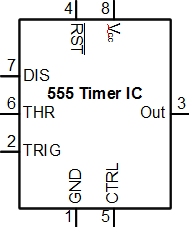
\includegraphics[width=1.2992in,height=1.5591in]{figures/ee4document-img004.png} 

{\selectlanguage{english}\sffamily\bfseries\color[rgb]{0.30980393,0.5058824,0.7411765}
Figure 10 Example schematic symbol for a 555 timer IC}

{\selectlanguage{english}\sffamily\color[rgb]{0.30980393,0.5058824,0.7411765}
The \textbf{schematic symbol} represents your component in the schematic editor. At the simplest level, it is a connect
of pins (representing the physical device pins) which you can connect wires to on your schematic.}

{\selectlanguage{english}\sffamily\color[rgb]{0.30980393,0.5058824,0.7411765}
In addition to the pins, it is common practice to include the component's electrical symbol. While symbols exist for
common parts like resistors, capacitors, inductors, and diodes, there are often no symbols for the pletora of chips. In
those cases, a the component is represented by a box with pins on the edges (like in the 555 timer above).}


\bigskip

{\selectlanguage{english}\sffamily\color[rgb]{0.30980393,0.5058824,0.7411765}
Additionally, it is common practice to arrange pins such that things {\textquotedbl}flow{\textquotedbl} from left to
right - with inputs on the left and outputs on the right. However, it is also common to lay out component symbols so
that pins correspond to the locations on the actual device.}


\bigskip

\subsubsection{Component footprints / patterns}
\hypertarget{Toc337742692}{} 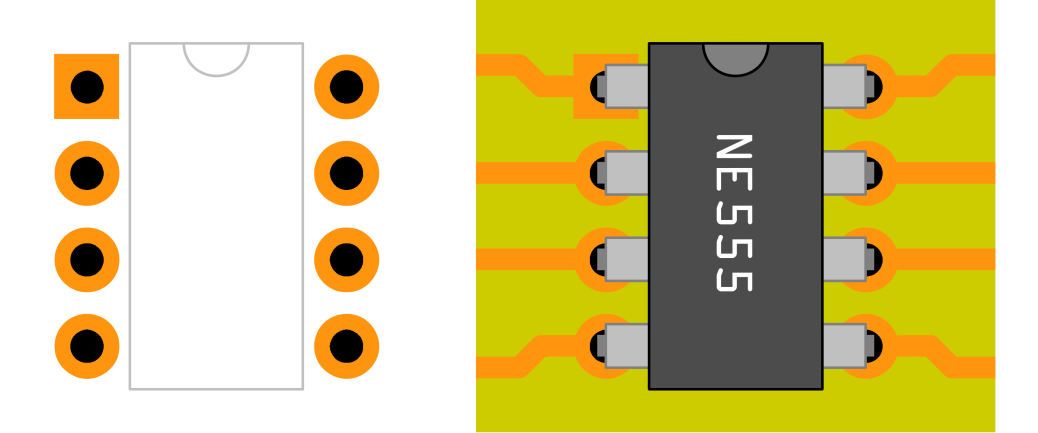
\includegraphics[width=4.7189in,height=1.9681in]{figures/ee4document-img015.png} 

{\selectlanguage{english}\sffamily\bfseries\color[rgb]{0.30980393,0.5058824,0.7411765}
Figure 10 Example 555 timer pattern (left, silkscreen in grey) and actual layout (right)}

{\selectlanguage{english}\sffamily\color[rgb]{0.30980393,0.5058824,0.7411765}
The \textbf{component footprint or pattern} defines the arrangement of pads and silkscreen patterns necessary to attach
a component to the circuit board.}

{\selectlanguage{english}\sffamily\color[rgb]{0.30980393,0.5058824,0.7411765}
\textbf{Pads} define the board features (copper and drill holes) to which the component will be attached. Usually, there
is one pad for each component pin.}

{\selectlanguage{english}\sffamily\color[rgb]{0.30980393,0.5058824,0.7411765}
Pad holes are usually only necessary for through-hole components or mounting pins. When a through-hole pad is required,
the copper pattern is repeated on both the top and bottom layer. Circular or ellipsoidal copper patterns are the most
common for these, although a square patterns are commonly used to indicate pin 1 for through-hole components.}

{\selectlanguage{english}\sffamily\color[rgb]{0.30980393,0.5058824,0.7411765}
Drill holes in pads are always plated. It is possible to get non-plated holes (\textbf{mounting holes}) on components,
but this usually increases fabrication cost and is replaced with a plated hole where possible.}

{\selectlanguage{english}\sffamily\color[rgb]{0.30980393,0.5058824,0.7411765}
The silkscreen layer usually includes a place for the component's refdes. Any information for aligning polarized
components are also included - usually this is a dot next to the first pin for ICs, and a bar on the cathode terminal
for diodes. }

\clearpage
\bigskip

\section{Parts List}
\hypertarget{Toc337742693}{}\begin{flushleft}
\tablefirsthead{}
\tablehead{}
\tabletail{}
\tablelasttail{}
\begin{supertabular}{|m{1.4247599in}|m{1.9212599in}|m{1.9212599in}|m{1.9247599in}|}
\hline
{\selectlanguage{english}\sffamily\bfseries\color[rgb]{0.30980393,0.5058824,0.7411765} Item} &
{\selectlanguage{english}\sffamily\bfseries\color[rgb]{0.30980393,0.5058824,0.7411765} Image} &
{\selectlanguage{english}\sffamily\color[rgb]{0.30980393,0.5058824,0.7411765} \textbf{Function}} &
{\selectlanguage{english}\sffamily\bfseries\color[rgb]{0.30980393,0.5058824,0.7411765} Notes}\\\hline
{\selectlanguage{english}\sffamily\color[rgb]{0.30980393,0.5058824,0.7411765} Your laptop} &
 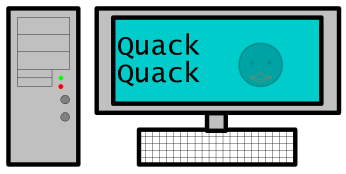
\includegraphics[width=1.5728in,height=0.7909in]{figures/ee4document-img016.png} 
{\selectlanguage{english}\sffamily\color[rgb]{0.30980393,0.5058824,0.7411765} (please \textit{don't} bring a desktop)} &
{\selectlanguage{english}\sffamily\color[rgb]{0.30980393,0.5058824,0.7411765} To run the software.} &
{\selectlanguage{english}\sffamily\color[rgb]{0.30980393,0.5058824,0.7411765} This isn't a parts-heavy lab, since it
only deals with design}\\\hline
\end{supertabular}
\end{flushleft}
\section{Lab Manual}
\hypertarget{Toc337742694}{}{\selectlanguage{english}\sffamily\color[rgb]{0.30980393,0.5058824,0.7411765}
What follows is a quick crash course in using DipTrace. Not all features will be explored - rather, only the basics will
be touched upon. For more information, consider working through the official DipTrace tutorial:
http://diptrace.com/books/tutorial.pdf (218 pages, lots of pictures.)}


\bigskip

{\selectlanguage{english}\sffamily\color[rgb]{0.30980393,0.5058824,0.7411765}
Also, note that a lot of this tutorial depends on your intuition with design software. Things like the mouse button and
some keyboard commands (especially the delete and escape button) do what you would expect them to do.}


\bigskip

\subsection{Lab 3.0: Pre-lab: setup and circuit overview}
\hypertarget{Toc337742695}{}{\selectlanguage{english}\sffamily\color[rgb]{0.30980393,0.5058824,0.7411765}
In CalSol, the PCB design suite we use is DipTrace (\url{http://www.diptrace.com/}), as we have the full version
sponsored. All of the boards on Impulse were laid out using DipTrace, and if you have Dropbox access, you can view
them.}


\bigskip

\liststyleRTFNumvi
\begin{enumerate}
\item {\selectlanguage{english}\sffamily\color[rgb]{0.30980393,0.5058824,0.7411765}
Install DipTrace}
\end{enumerate}

\bigskip

\clearpage
\bigskip

\subsection{Lab 3.1: Circuit design}
\hypertarget{Toc337742696}{}{\selectlanguage{english}\sffamily\color[rgb]{0.30980393,0.5058824,0.7411765}
If you did the Extra for Experts during EE1, you will be familiar with the 555 timer circuit. Basically, it uses a 555
timer chip (along with some supporting components) to blink an LED.}

 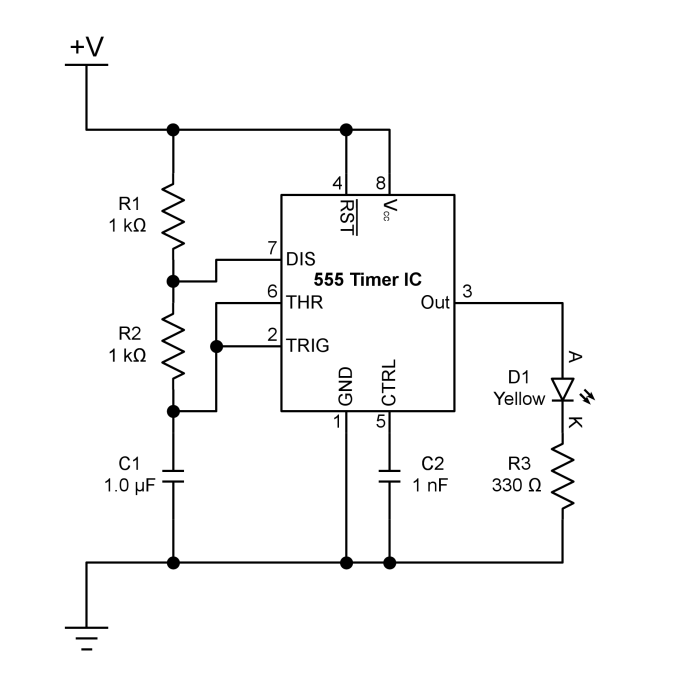
\includegraphics[width=3.15in,height=3.15in]{figures/ee4document-img017.png} 

{\selectlanguage{english}\sffamily\bfseries\color[rgb]{0.30980393,0.5058824,0.7411765}
Figure 10 The 555 timer circuit}

{\selectlanguage{english}\sffamily\color[rgb]{0.30980393,0.5058824,0.7411765}
Today, we will be designing a board around this circuit.}

\subsection{Lab 3.2: Schematic entry}
\hypertarget{Toc337742697}{}{\selectlanguage{english}\sffamily\color[rgb]{0.30980393,0.5058824,0.7411765}
Enter the circuit into the DipTrace schematic editor.}


\bigskip

\liststyleRTFNumvi
\setcounter{saveenum}{\value{enumi}}
\begin{enumerate}
\setcounter{enumi}{\value{saveenum}}
\item {\selectlanguage{english}\sffamily\color[rgb]{0.30980393,0.5058824,0.7411765}
Start up DipTrace Schematic.\newline
 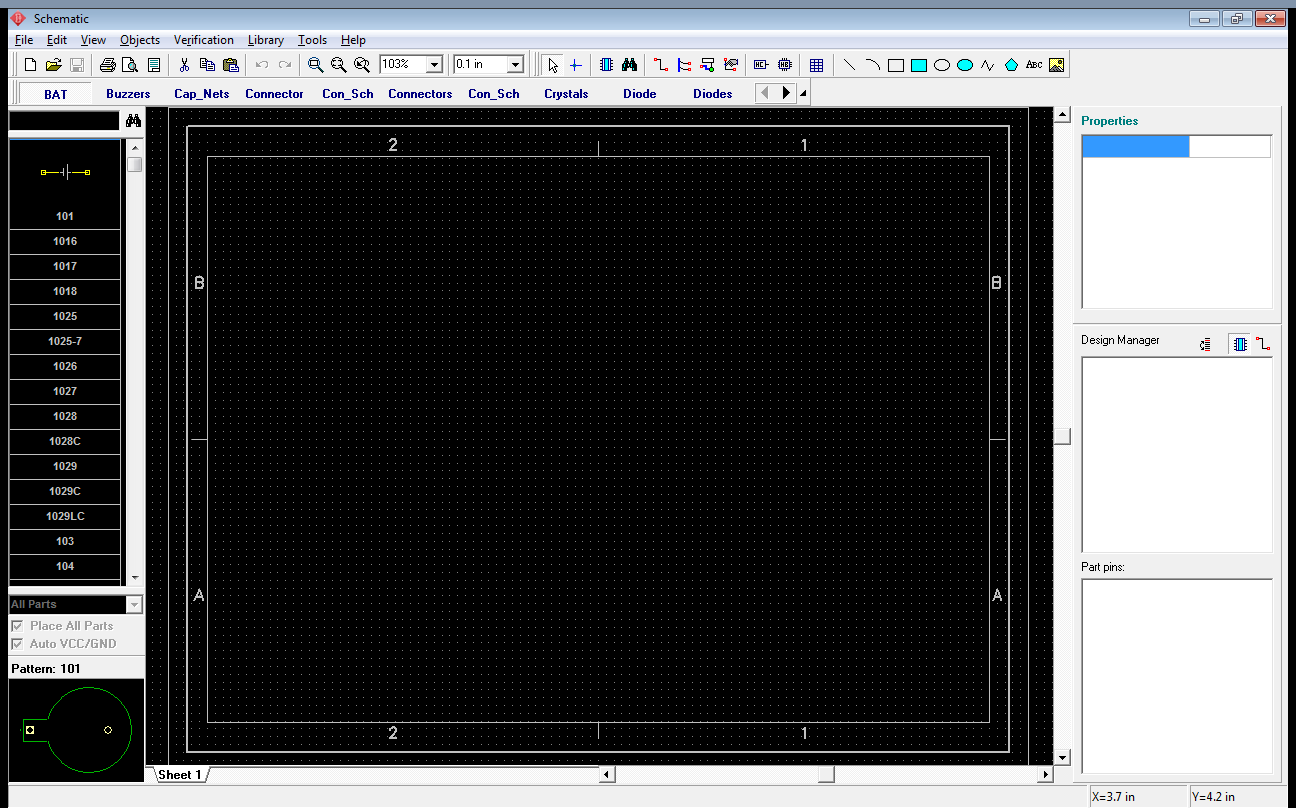
\includegraphics[width=5.4in,height=3.3665in]{figures/ee4document-img018.png} }
\item {\selectlanguage{english}\sffamily\color[rgb]{0.30980393,0.5058824,0.7411765}
Play around with the interface.\newline
In the main view of the schematic, you can use the mouse wheel to zoom in and out.\newline
On the left side of the screen is where you can view components in the current library.\newline
You can select the current library using the buttons below the toolbar.}
\item {\selectlanguage{english}\sffamily\color[rgb]{0.30980393,0.5058824,0.7411765}
On the library selection bar, scroll right and select the {\textquotedbl}National{\textquotedbl} tab. The listing of
components should change accordingly.}
\item {\selectlanguage{english}\sffamily\color[rgb]{0.30980393,0.5058824,0.7411765}
On the listing of components, select the LMC555CN. This should allow you to place the component}
\end{enumerate}
{\selectlanguage{english}\sffamily\color[rgb]{0.30980393,0.5058824,0.7411765}
Go to an empty space on your schematic, and place the component by clicking the left mouse button.\newline
 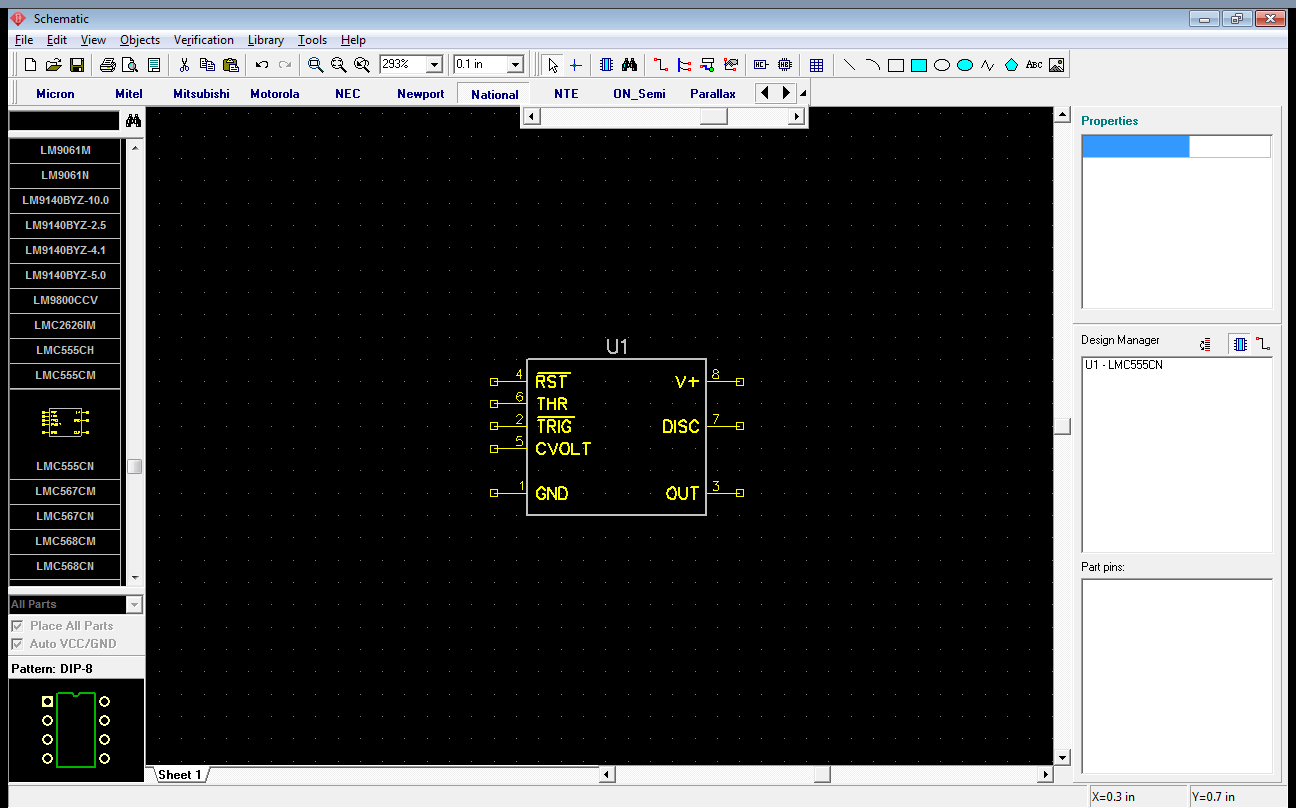
\includegraphics[width=5.4in,height=3.3665in]{figures/ee4document-img019.png} }

{\selectlanguage{english}\sffamily\color[rgb]{0.30980393,0.5058824,0.7411765}
However, there are other ways to select components. Go to the main menu, and select Objects-{\textgreater}Place
Component. The Place Component dialog should come up.}

\liststyleRTFNumvi
\setcounter{saveenum}{\value{enumi}}
\begin{enumerate}
\setcounter{enumi}{\value{saveenum}}
\item \setcounter{saveenum}{\value{enumii}}
\begin{enumerate}
\setcounter{enumii}{\value{saveenum}}
\item {\selectlanguage{english}\sffamily\color[rgb]{0.30980393,0.5058824,0.7411765}
The list of loaded libraries is initially empty, so click {\textquotedbl}Add{\textquotedbl}, and select
{\textquotedbl}\_discrete.eli{\textquotedbl} from the file selection window.}
\item {\selectlanguage{english}\sffamily\color[rgb]{0.30980393,0.5058824,0.7411765}
Select the Discrete library from the list. This should populate the list on the right with the components in that
library.}
\end{enumerate}
\end{enumerate}
{\selectlanguage{english}\sffamily\color[rgb]{0.30980393,0.5058824,0.7411765}
What we're interested in is a resistor. Type {\textquotedbl}RES400{\textquotedbl} (a 400 mil spacing resistor) into the
search bar, and click {\textquotedbl}Search.{\textquotedbl} One component should be left.\newline
 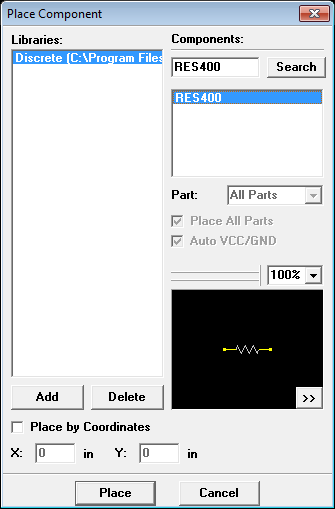
\includegraphics[width=1.3957in,height=2.1209in]{figures/ee4document-img020.png} }

{\selectlanguage{english}\sffamily\color[rgb]{0.30980393,0.5058824,0.7411765}
Select that component, and click {\textquotedbl}Place.{\textquotedbl}}

{\selectlanguage{english}\sffamily\color[rgb]{0.30980393,0.5058824,0.7411765}
Place the component on your schematic. You may need several resistors.}

{\selectlanguage{english}\sffamily\color[rgb]{0.30980393,0.5058824,0.7411765}
For each resistor, you need to set component specific information, like its value (resistance, in this case.) Double
click the resistor, and set its Value in the component properties. Alternatively, you can select the component and edit
its property sheet on the right.}

\liststyleRTFNumvi
\setcounter{saveenum}{\value{enumi}}
\begin{enumerate}
\setcounter{enumi}{\value{saveenum}}
\item {\selectlanguage{english}\sffamily\color[rgb]{0.30980393,0.5058824,0.7411765}
You can wire your components by clicking on the small box on the component's terminal. Then, once you have reached the
destination pin, click again to finalize the wire.}
\item {\selectlanguage{english}\sffamily\color[rgb]{0.30980393,0.5058824,0.7411765}
Also, place the required LEDs and capacitors. The LEDs are in the {\textquotedbl}Discrete{\textquotedbl} library and
named {\textquotedbl}LED.{\textquotedbl} The capacitor is also in the {\textquotedbl}Discrete{\textquotedbl} library,
and named {\textquotedbl}CAP100.{\textquotedbl}}

\setcounter{saveenum}{\value{enumii}}
\begin{enumerate}
\setcounter{enumii}{\value{saveenum}}
\item {\selectlanguage{english}\sffamily\color[rgb]{0.30980393,0.5058824,0.7411765}
By now, you will probably have quite a few components. If you right click a component, you can see what you can do with
them. Rotating and flipping them may help you organize your schematic.}
\end{enumerate}
\item {\selectlanguage{english}\sffamily\color[rgb]{0.30980393,0.5058824,0.7411765}
Don't forget to add the power supplies. Remember from the technical manual that all the power supply symbols are
connected. For this chip, add both a ground and a 5v power supply. The relevant symbols are in the
{\textquotedbl}Disc\_Sch{\textquotedbl} library.}
\item {\selectlanguage{english}\sffamily\color[rgb]{0.30980393,0.5058824,0.7411765}
You may need to be creative with arranging your schematic to keep it readable. One possible schematic diagram is shown
here:\newline
 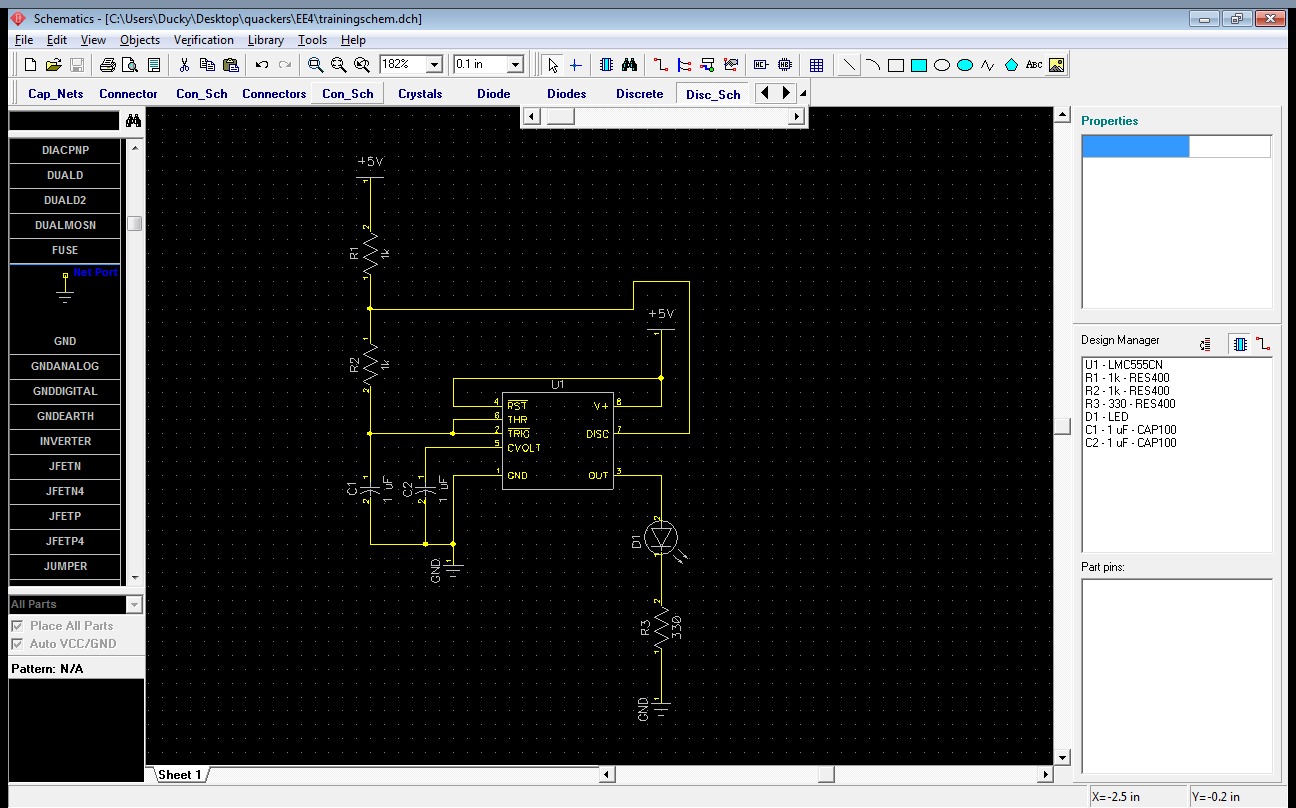
\includegraphics[width=5.4in,height=3.3665in]{figures/ee4document-img021.png} \newline
 }
\end{enumerate}
\subsection{Lab 3.3: Layout}
\hypertarget{Toc337742698}{}{\selectlanguage{english}\sffamily\color[rgb]{0.30980393,0.5058824,0.7411765}
Convert the schematic into a board, and layout the components and traces.}

\liststyleRTFNumvi
\setcounter{saveenum}{\value{enumi}}
\begin{enumerate}
\setcounter{enumi}{\value{saveenum}}
\item {\selectlanguage{english}\sffamily\color[rgb]{0.30980393,0.5058824,0.7411765}
In the schematic editor's main menu, click File-{\textgreater}Convert to PCB. Your circuit should now \ appear in the
PCB Layout tool.\newline
 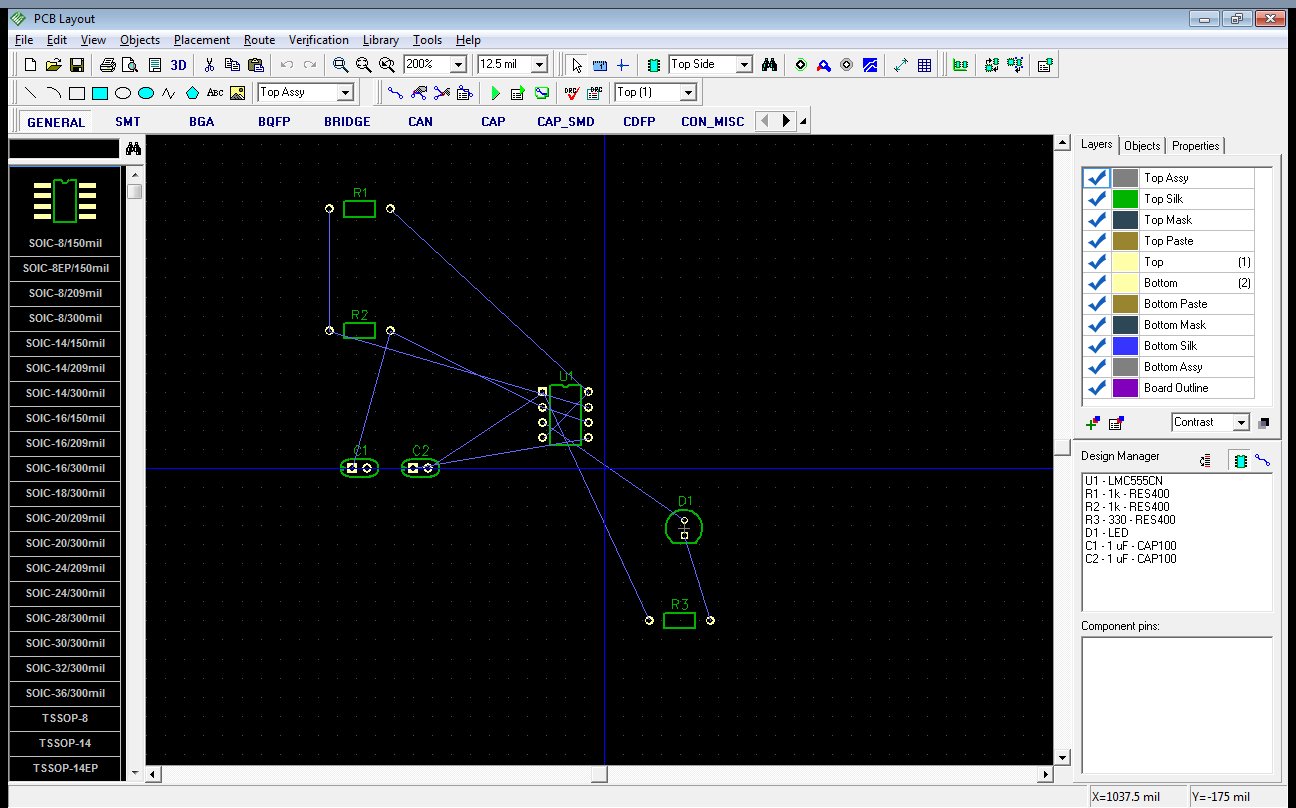
\includegraphics[width=5.4in,height=3.3665in]{figures/ee4document-img022.png} }
\end{enumerate}
{\selectlanguage{english}\sffamily\color[rgb]{0.30980393,0.5058824,0.7411765}
Start off by checking the layout settings. For this project, you can set your grid at 100 mil. The grid settings are on
the top bar.}

{\selectlanguage{english}\sffamily\color[rgb]{0.30980393,0.5058824,0.7411765}
Also, set up the design rules in Verification-{\textgreater}Design Rules.}

\liststyleRTFNumvi
\setcounter{saveenum}{\value{enumi}}
\begin{enumerate}
\setcounter{enumi}{\value{saveenum}}
\item \setcounter{saveenum}{\value{enumii}}
\begin{enumerate}
\setcounter{enumii}{\value{saveenum}}
\item {\selectlanguage{english}\sffamily\color[rgb]{0.30980393,0.5058824,0.7411765}
The table you see defines the feature-to-feature minimum spacings. 8 mil should be adequate.\newline
 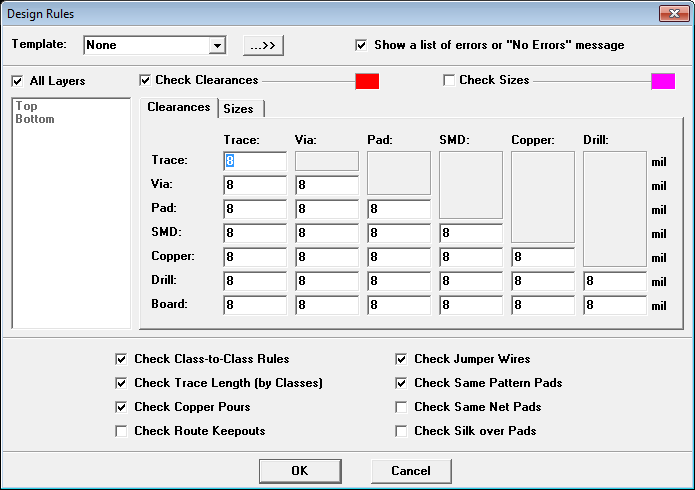
\includegraphics[width=2.8957in,height=2.0417in]{figures/ee4document-img023.png} }
\end{enumerate}
\end{enumerate}
{\selectlanguage{english}\sffamily\color[rgb]{0.30980393,0.5058824,0.7411765}
Also, check the sizes. 8 mil should be good for minimum trace width, and 20 mil should be good for the minimum drill
size.\newline
 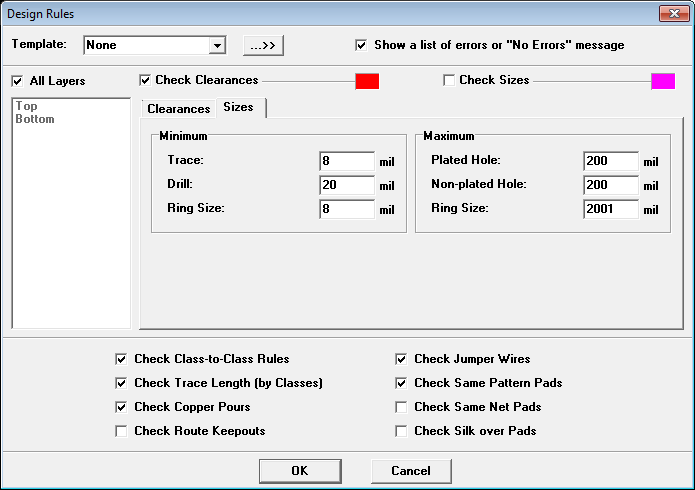
\includegraphics[width=2.8957in,height=2.0417in]{figures/ee4document-img024.png} }

{\selectlanguage{english}\sffamily\color[rgb]{0.30980393,0.5058824,0.7411765}
Yes, we can go lower if you really need it - 6 mil trace width / spacing and 15mil minimum drill size is the limit. But
we won't - it's not a good idea to design at the limits.}

\liststyleRTFNumvi
\setcounter{saveenum}{\value{enumi}}
\begin{enumerate}
\setcounter{enumi}{\value{saveenum}}
\item {\selectlanguage{english}\sffamily\color[rgb]{0.30980393,0.5058824,0.7411765}
Now, you should probably define the board outline. Let's say that you want a 2 square inch board. In the main menu,
click Object-{\textgreater}Place Board Outline. Click on the schematic to define the points on your board outline. Once
you form a closed polygon, the board outline will have been defined.}
\item {\selectlanguage{english}\sffamily\color[rgb]{0.30980393,0.5058824,0.7411765}
Move components around in preparation for layout. Do this by clicking and dragging the components. Again, you can rotate
components by right clicking on them and selecting {\textquotedbl}Rotate,{\textquotedbl} or by pressing Ctrl + R.}
\end{enumerate}
{\selectlanguage{english}\sffamily\color[rgb]{0.30980393,0.5058824,0.7411765}
Route your design.\newline
 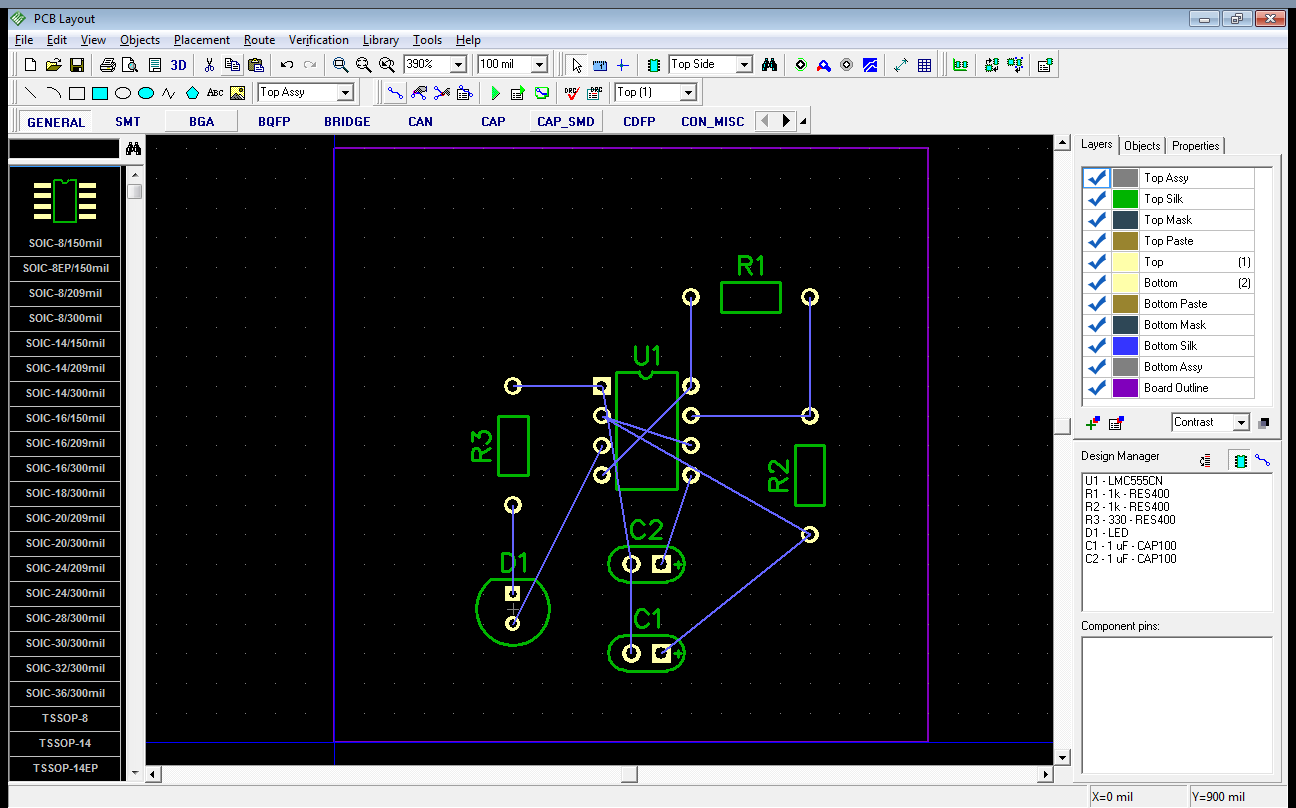
\includegraphics[width=13.5in,height=0.252in]{figures/ee4document-img025.png} }

\liststyleRTFNumvi
\setcounter{saveenum}{\value{enumi}}
\begin{enumerate}
\setcounter{enumi}{\value{saveenum}}
\item \setcounter{saveenum}{\value{enumii}}
\begin{enumerate}
\setcounter{enumii}{\value{saveenum}}
\item {\selectlanguage{english}\sffamily\color[rgb]{0.30980393,0.5058824,0.7411765}
Click the {\textquotedbl}Route Setup{\textquotedbl} button on the toolbar, and set your routing trace width. Let's set
it at 15 mil trace width.}
\item {\selectlanguage{english}\sffamily\color[rgb]{0.30980393,0.5058824,0.7411765}
Enter routing mode by clicking the {\textquotedbl}Route Manual{\textquotedbl} button on the toolbar.}
\item {\selectlanguage{english}\sffamily\color[rgb]{0.30980393,0.5058824,0.7411765}
You can place routes by clicking on a pad. Click to set down a routed segment. Routing of a particular trace ends on
either a double-click or when it hits a connected pad.}
\item {\selectlanguage{english}\sffamily\color[rgb]{0.30980393,0.5058824,0.7411765}
You probably don't want to try routing everything on just one layer. Press (1) and (2) to switch between the two copper
layers. Doing this in the middle of a routing operation will create a via to connect the two layers.}
\item {\selectlanguage{english}\sffamily\color[rgb]{0.30980393,0.5058824,0.7411765}
An example routed design is below:\newline
 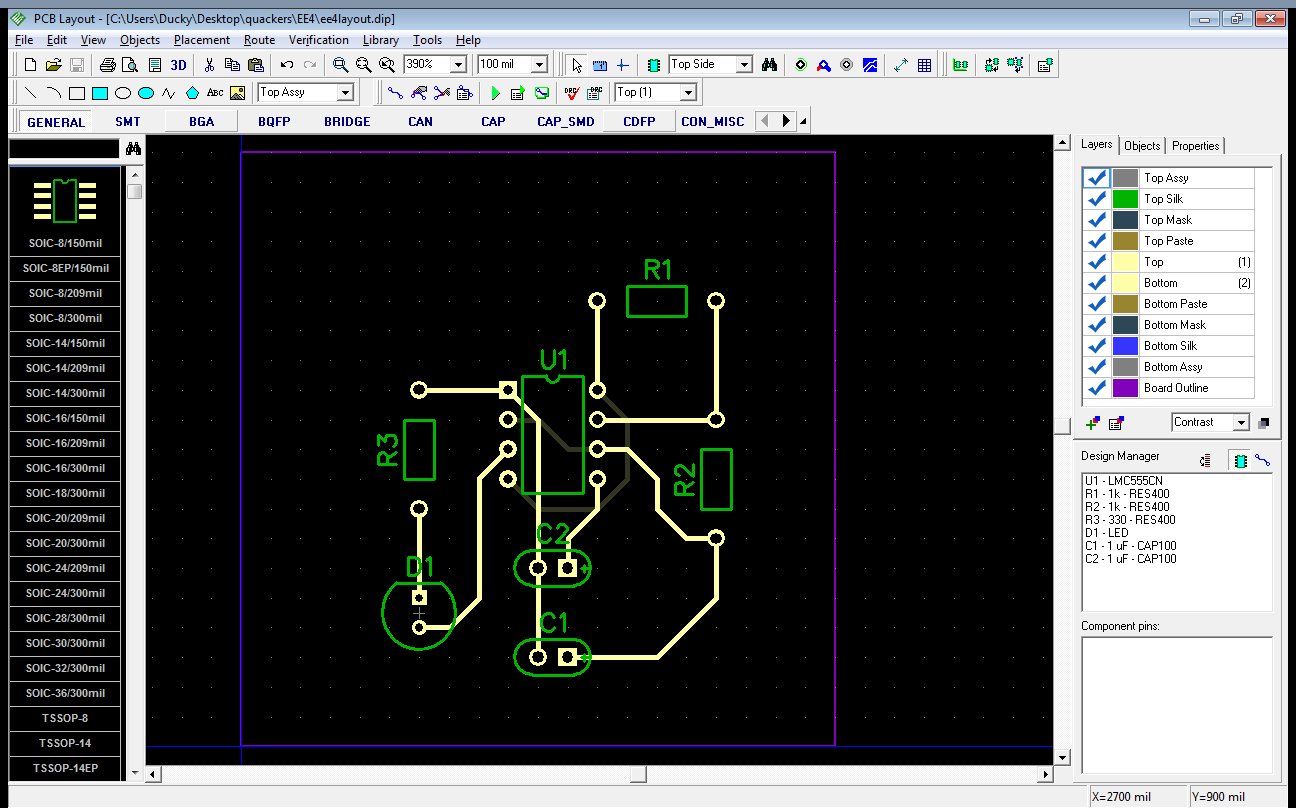
\includegraphics[width=5.4in,height=3.3665in]{figures/ee4document-img026.png} }
\end{enumerate}
\end{enumerate}

\bigskip

\subsection{Lab 3.4: Forward annotation}
\hypertarget{Toc337742699}{}{\selectlanguage{english}\sffamily\color[rgb]{0.30980393,0.5058824,0.7411765}
Rarely do you get your schematic right on the first try. \textbf{Forward annotation} is updating an existing layout with
a new schematic version.}


\bigskip

\liststyleRTFNumvi
\setcounter{saveenum}{\value{enumi}}
\begin{enumerate}
\setcounter{enumi}{\value{saveenum}}
\item {\selectlanguage{english}\sffamily\color[rgb]{0.30980393,0.5058824,0.7411765}
It turns out we forgot our power supply! Uh-oh! Go back to the schematic editor, and let's correct this major
oversight.}
\item {\selectlanguage{english}\sffamily\color[rgb]{0.30980393,0.5058824,0.7411765}
In the component library {\textquotedbl}BAT,{\textquotedbl} place the component {\textquotedbl}BS-7{\textquotedbl} (a
CR2032 coin cell holder) on your schematic. Connect +5v and ground to it. Note that batteries are polarized devices,
and the longer line on the schematic symbol indicates the positive terminal.}
\item {\selectlanguage{english}\sffamily\color[rgb]{0.30980393,0.5058824,0.7411765}
A possible schematic looks like this:\newline
 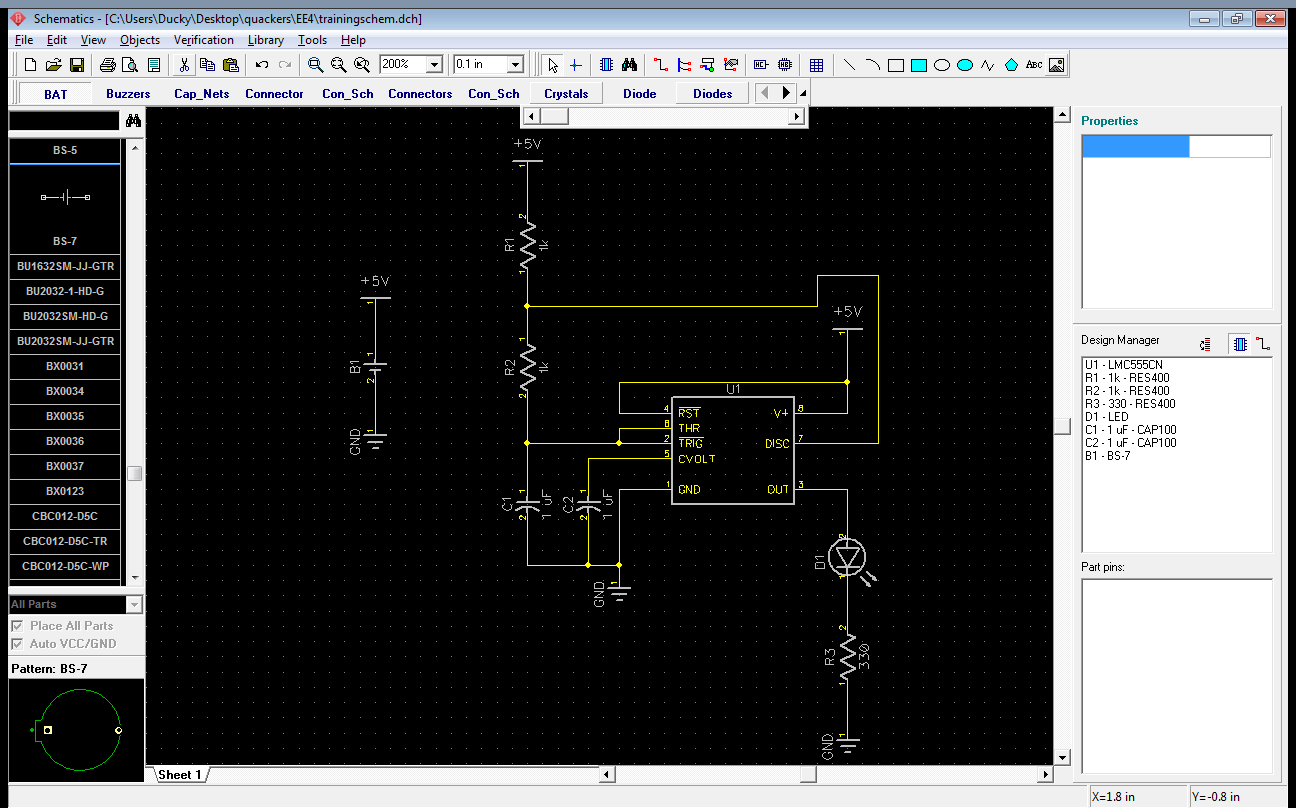
\includegraphics[width=5.4in,height=3.3665in]{figures/ee4document-img027.png} \newline
Notice how the battery is only implicitly connected to the rest of the schematic using the power components.\newline
}
\item {\selectlanguage{english}\sffamily\color[rgb]{0.30980393,0.5058824,0.7411765}
Now, update your circuit board design with the new schematic. In the PCB layout editor, click File-{\textgreater}Renew
Design from Schematic-{\textgreater}By Component, and select your schematic file.}
\item {\selectlanguage{english}\sffamily\color[rgb]{0.30980393,0.5058824,0.7411765}
Route the new battery holder component. Feel free to change your board dimensions as necessary (you can click on the
board outline and drag the points.) One possible layout is as follows:\newline
 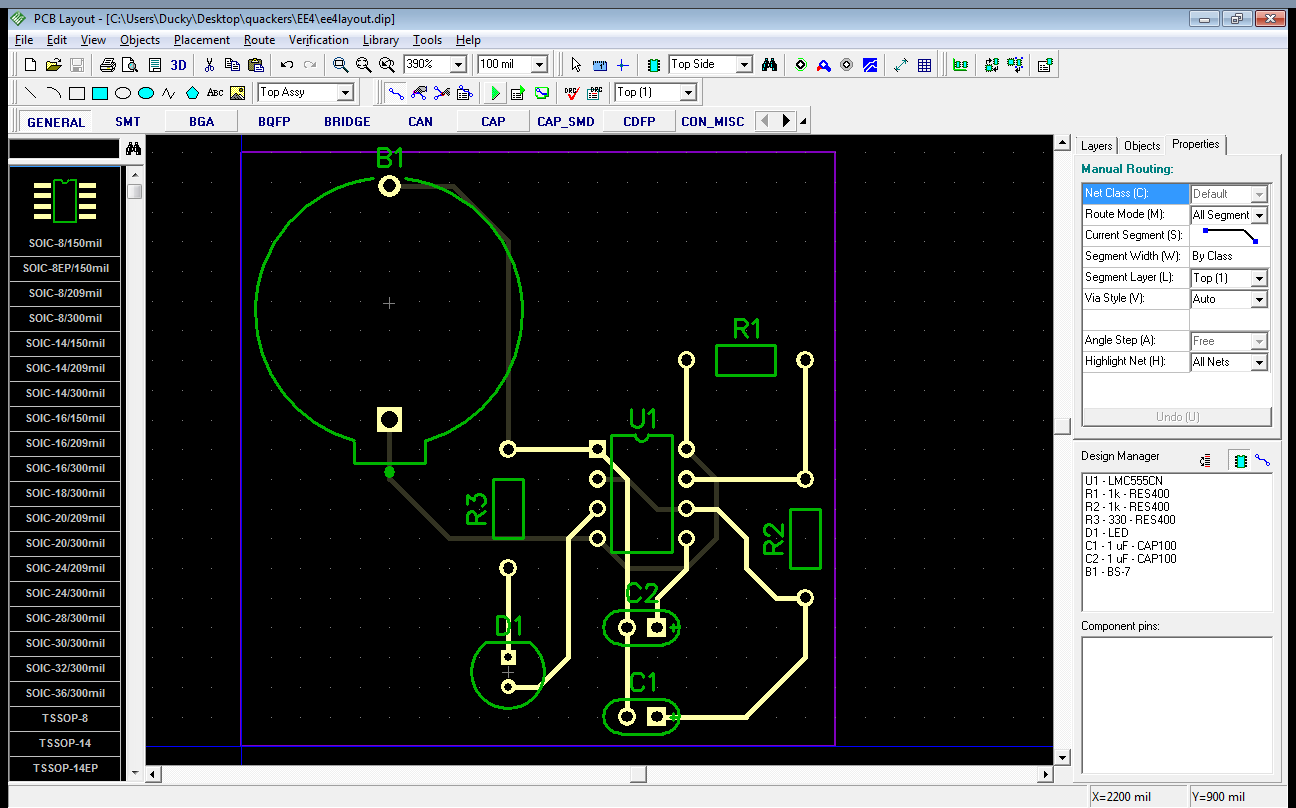
\includegraphics[width=5.4in,height=3.3665in]{figures/ee4document-img028.png} }
\end{enumerate}

\bigskip

\subsection[Lab 3.5: Design verification]{Lab 3.5: Design verification}
\hypertarget{Toc337742700}{}{\selectlanguage{english}\sffamily\color[rgb]{0.30980393,0.5058824,0.7411765}
Your design is complete. But, does it work?}


\bigskip

\liststyleRTFNumvi
\setcounter{saveenum}{\value{enumi}}
\begin{enumerate}
\setcounter{enumi}{\value{saveenum}}
\item {\selectlanguage{english}\sffamily\color[rgb]{0.30980393,0.5058824,0.7411765}
First, check that your design is completely routed. In the menu, click Verification-{\textgreater}Check Net
Connectivity. Accept the default settings (the checker will take into consideration copper traces, shapes, and pours),
and let it check your layout. If you routed your board correctly, it should say {\textquotedbl}no errors
found.{\textquotedbl} Otherwise, you need to go back and fix any mistakes you made.}
\item {\selectlanguage{english}\sffamily\color[rgb]{0.30980393,0.5058824,0.7411765}
Similarly, check that you have satisfied all the design rules - click Verification-{\textgreater}Check Design Rules, or
F9. If it passes, it will tell you {\textquotedbl}no errors found,{\textquotedbl} otherwise, it will indicate where you
messed up.}
\item {\selectlanguage{english}\sffamily\color[rgb]{0.30980393,0.5058824,0.7411765}
On a real design, it's always a good idea to get both your schematic and layout checked by another person.}
\end{enumerate}

\bigskip

\subsection{Lab 3.6: Fabrication data}
\hypertarget{Toc337742701}{}{\selectlanguage{english}\sffamily\color[rgb]{0.30980393,0.5058824,0.7411765}
Most board houses will only accept Gerber files for fabrication - they do not have the time to deal with all the
different file formats created by all the different programs. You need to generate these files once your board design
is complete.}


\bigskip

\liststyleRTFNumvi
\setcounter{saveenum}{\value{enumi}}
\begin{enumerate}
\setcounter{enumi}{\value{saveenum}}
\item {\selectlanguage{english}\sffamily\color[rgb]{0.30980393,0.5058824,0.7411765}
Export a complete set of Gerbers. Go to File-{\textgreater}Export-{\textgreater}Gerbers.}

\setcounter{saveenum}{\value{enumii}}
\begin{enumerate}
\setcounter{enumii}{\value{saveenum}}
\item {\selectlanguage{english}\sffamily\color[rgb]{0.30980393,0.5058824,0.7411765}
The default settings should work fine. Click {\textquotedbl}Export All,{\textquotedbl} and give those Gerber files a
home.}
\item {\selectlanguage{english}\sffamily\color[rgb]{0.30980393,0.5058824,0.7411765}
DipTrace will export more Gerber files than you need. The only essential ones for PCB fabrication are the copper layers,
the soldermask layers, the silkscreen layers, and the board outline.}
\end{enumerate}
\item {\selectlanguage{english}\sffamily\color[rgb]{0.30980393,0.5058824,0.7411765}
Export the NC drill file. Go to File-{\textgreater}Export-{\textgreater}N/C Drill.}

\setcounter{saveenum}{\value{enumii}}
\begin{enumerate}
\setcounter{enumii}{\value{saveenum}}
\item {\selectlanguage{english}\sffamily\color[rgb]{0.30980393,0.5058824,0.7411765}
Again, the default settings should be fine. Click {\textquotedbl}Export,{\textquotedbl} and save the file in the same
folder.}
\end{enumerate}
\end{enumerate}
\clearpage
\bigskip

\liststyleRTFNumvi
\setcounter{saveenum}{\value{enumi}}
\begin{enumerate}
\setcounter{enumi}{\value{saveenum}}
\item {\selectlanguage{english}\sffamily\color[rgb]{0.30980393,0.5058824,0.7411765}
Usually, you want to verify that your Gerbers are, in fact, sane.}
\end{enumerate}
{\selectlanguage{english}\sffamily\color[rgb]{0.30980393,0.5058824,0.7411765}
Dedicated Gerber viewer programs exist. Check out gerbv and see if you can get it to open your freshly created Gerber
files.\newline
 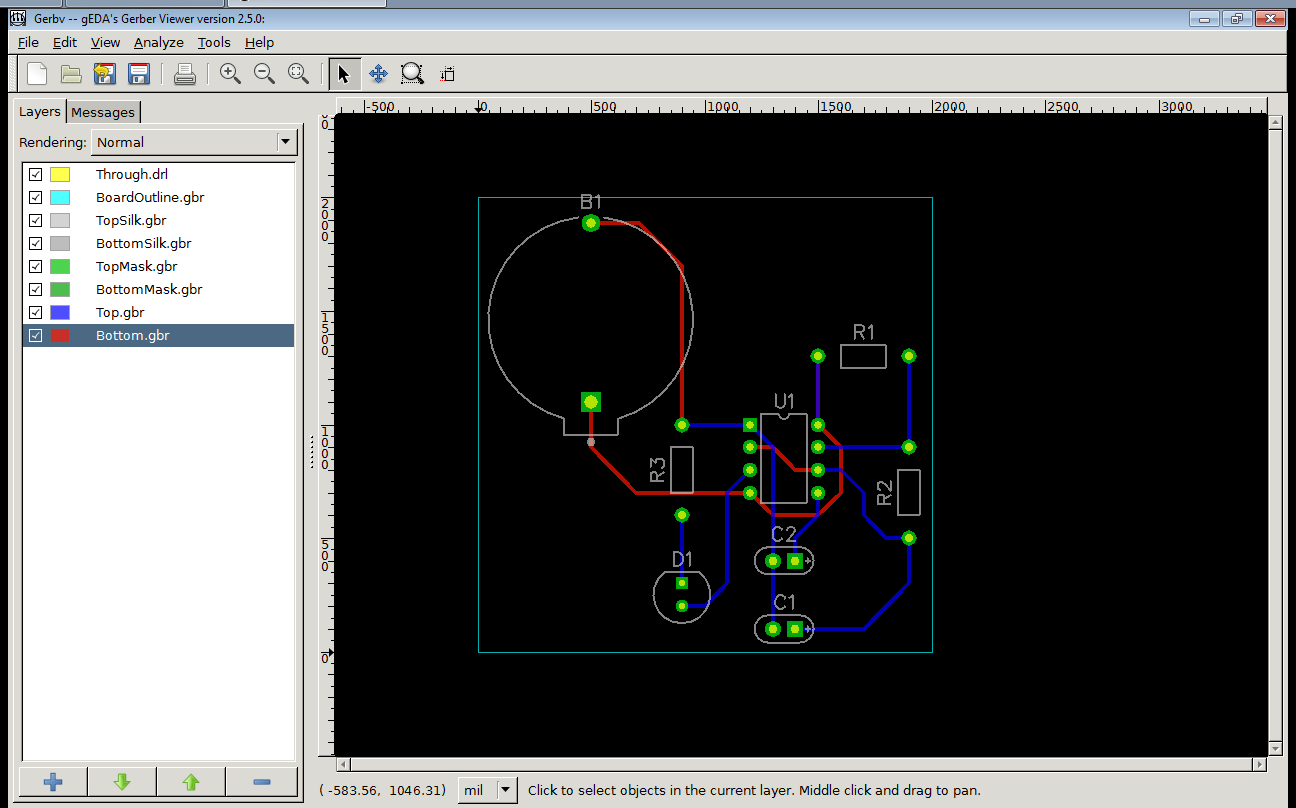
\includegraphics[width=5.4in,height=3.3665in]{figures/ee4document-img029.png} }

{\selectlanguage{english}\sffamily\color[rgb]{0.30980393,0.5058824,0.7411765}
Otherwise, if your board house has an online submission process, it \textit{may} display your board files before your
confirm your order.}

\liststyleRTFNumvi
\setcounter{saveenum}{\value{enumi}}
\begin{enumerate}
\setcounter{enumi}{\value{saveenum}}
\item {\selectlanguage{english}\sffamily\color[rgb]{0.30980393,0.5058824,0.7411765}
Congratulations. You've created your first circuit board.}
\end{enumerate}

\bigskip

\clearpage
\bigskip

\subsection{Lab 3.7: Extra for Experts: Component creation \& surface mount}
\hypertarget{Toc337742702}{}{\selectlanguage{english}\sffamily\color[rgb]{0.30980393,0.5058824,0.7411765}
Say that you don't like that boring 5mm LED. You want something a little more powerful. Scratch that, you want something
\textit{blindingly} powerful - 100+ lumens powerful. Something like a 1 watt LED\footnote{\ You will not reach the full
power output of the LED by using only the 555 timer - it sources at most 150mA. You will need a transistor amplifier to
use the LED to its full, blinding, potential.} \footnote{\ It is also unlikely that the small coin cell battery can
supply all the current required for the LED. The design will likely need a larger battery or a dedicated power
supply.}.}

{\selectlanguage{english}\sffamily\bfseries\color[rgb]{0.30980393,0.5058824,0.7411765}
Digikey link:}

{\selectlanguage{english}\sffamily\color[rgb]{0.30980393,0.5058824,0.7411765}
\url{http://search.digikey.com/us/en/products/MX3AWT-A1-R250-000CE3/MX3AWT-A1-R250-000CE3CT-ND/2356708}}

{\selectlanguage{english}\sffamily\bfseries\color[rgb]{0.30980393,0.5058824,0.7411765}
Datasheet:}

{\selectlanguage{english}\sffamily\color[rgb]{0.30980393,0.5058824,0.7411765}
\url{http://www.cree.com/products/pdf/XLampMX-3.pdf}}


\bigskip

{\selectlanguage{english}\sffamily\color[rgb]{0.30980393,0.5058824,0.7411765}
However, no such component exists in the standard DipTrace libraries, so you'll have to create your own.}

\subsubsection{Pattern creation}
\hypertarget{Toc337742703}{}{\selectlanguage{english}\sffamily\color[rgb]{0.30980393,0.5058824,0.7411765}
So, where to start? With the recommended solder pattern, of course! Usually, on datasheets for parts, they will have a
recommended pattern, complete with dimensions. Your job is them to accurately input their drawing into the pattern
editor.}


\bigskip

\liststyleRTFNumxi
\begin{enumerate}
\item {\selectlanguage{english}\sffamily\color[rgb]{0.30980393,0.5058824,0.7411765}
Take a look at the recommended pattern. It is on page 8 of the component's datasheet.}

\begin{enumerate}
\item {\selectlanguage{english}\sffamily\color[rgb]{0.30980393,0.5058824,0.7411765}
Note that this is a surface-mount device. There are 2 electrically connected pins (anode and cathode) and a heatsink
pad.}
\item {\selectlanguage{english}\sffamily\color[rgb]{0.30980393,0.5058824,0.7411765}
The drawings may look a bit confusing at first - they have the hatched and clear boxes on the drawing. I believe the
hatched drawings are used for the stencil (indicates where to put solder paste) while the clear boxes are used to
indicate copper.}
\end{enumerate}
\item {\selectlanguage{english}\sffamily\color[rgb]{0.30980393,0.5058824,0.7411765}
Start the DipTrace pattern editor.\newline
 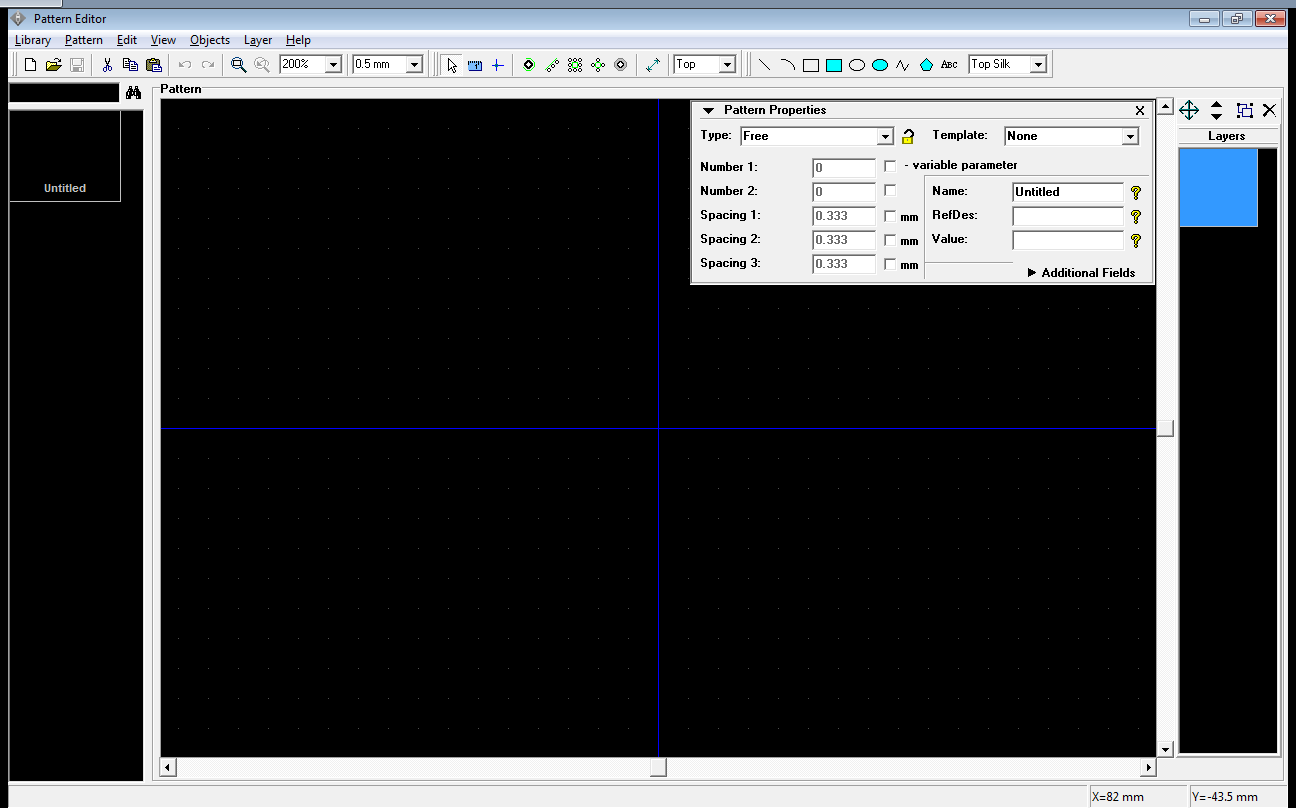
\includegraphics[width=5.4in,height=3.3665in]{figures/ee4document-img030.png} }
\end{enumerate}
{\selectlanguage{english}\sffamily\color[rgb]{0.30980393,0.5058824,0.7411765}
Ensure the pattern editor's units are set consistently with your component datasheet's units. The LED datasheet uses
millimeters, and you can set DipTrace's units by going to View-{\textgreater}Units.}

{\selectlanguage{english}\sffamily\color[rgb]{0.30980393,0.5058824,0.7411765}
The pattern editor defines a component's pattern with pads and shapes. You should already be familiar with pads from the
technical manual. As for shapes, it is just a geometric shape which can be placed on any layer, including silkscreen.}

{\selectlanguage{english}\sffamily\color[rgb]{0.30980393,0.5058824,0.7411765}
On the toolbox, click {\textquotedbl}Place Pad,{\textquotedbl} and place three pads anywhere on the schematic. Note that
your newly placed pads will NOT match what you want to do - this is fine (for now!)\newline
 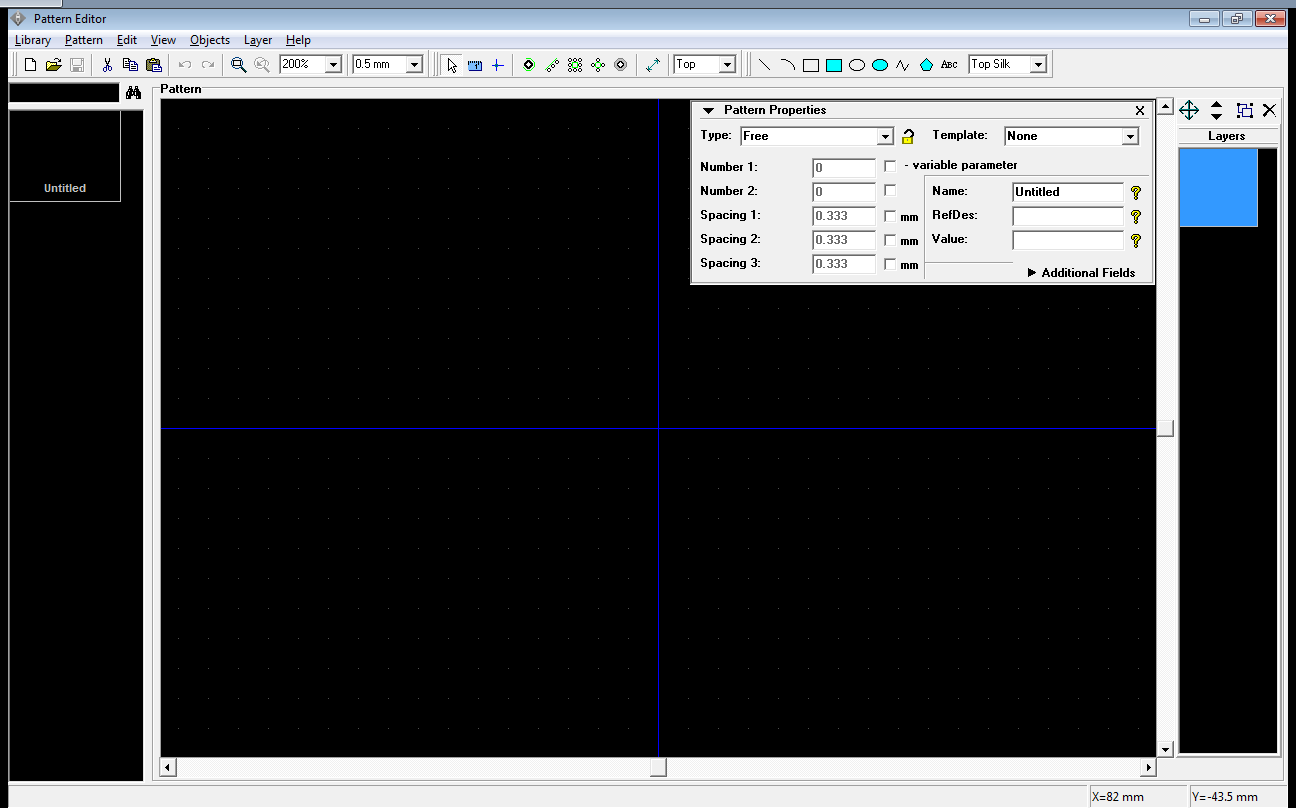
\includegraphics[width=1.2181in,height=0.3374in]{figures/ee4document-img030.png} }

{\selectlanguage{english}\sffamily\color[rgb]{0.30980393,0.5058824,0.7411765}
DipTrace defines pads with an  
\includegraphics[width=0.4272in,height=0.2083in]{figures/ee4document-img031.png}  coordinate, a
shape (rectangle, oval, circle, and polygon), and sizes. Define your pads according to the component datasheet.}

\liststyleRTFNumxi
\setcounter{saveenum}{\value{enumi}}
\begin{enumerate}
\setcounter{enumi}{\value{saveenum}}
\item \setcounter{saveenum}{\value{enumii}}
\begin{enumerate}
\setcounter{enumii}{\value{saveenum}}
\item {\selectlanguage{english}\sffamily\color[rgb]{0.30980393,0.5058824,0.7411765}
Note that the recommended pattern is more or less symmetrical along the horizontal axis. Therefore, you only need to
calculate the pad size for one side.}
\end{enumerate}
\end{enumerate}
{\selectlanguage{english}\sffamily\color[rgb]{0.30980393,0.5058824,0.7411765}
Calculate the pad size for either of the two outer pads.\newline
You should get  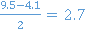
\includegraphics[width=0.8957in,height=0.302in]{figures/ee4document-img032.png}  mm for the width and 4.3mm for
the height. Make sure you understand how to get these numbers from the dimensioned drawing.}

{\selectlanguage{english}\sffamily\color[rgb]{0.30980393,0.5058824,0.7411765}
Choose any pad, and double-click it to bring up the properties. On the Type/Dimensions tab, ensure {\textquotedbl}Use
Pattern's Pad Properties{\textquotedbl} is checked, and edit the Pattern's Pad Properties. This sets the common pad
definition for the pattern.}

{\selectlanguage{english}\sffamily\color[rgb]{0.30980393,0.5058824,0.7411765}
Set the dimensions consistently with the numbers you got. You should be using a surface, rectangular pad without a
hole.\newline
 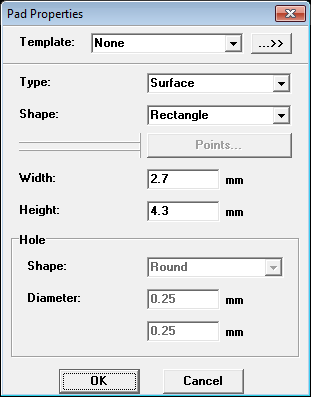
\includegraphics[width=1.2957in,height=1.6543in]{figures/ee4document-img033.png} \newline
If you were designing a through-hole component pad, you select a through-hole type pad, and set the hole size. In this
case, you must ensure that the hole is larger than the component pin and there is enough copper surrounding the hole to
satisfy design rules.}

{\selectlanguage{english}\sffamily\color[rgb]{0.30980393,0.5058824,0.7411765}
OK out of everything. All of your pads should have changed size now.}

{\selectlanguage{english}\sffamily\color[rgb]{0.30980393,0.5058824,0.7411765}
Calculate the X and Y position for the two outer pads. If you defined the origin of the pattern as the center of the
component, the  
\includegraphics[width=0.1043in,height=0.2083in]{figures/ee4document-img034.png}  coordinate should be
0.\newline
You should get  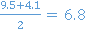
\includegraphics[width=0.8957in,height=0.302in]{figures/ee4document-img035.png}  mm as the distance between
centers and  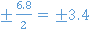
\includegraphics[width=0.9374in,height=0.302in]{figures/ee4document-img036.png}  mm as the 

\includegraphics[width=0.1043in,height=0.2083in]{figures/ee4document-img037.png}  coordinates.}

{\selectlanguage{english}\sffamily\color[rgb]{0.30980393,0.5058824,0.7411765}
Double-click the relevant pads (1 and 2) and input the 

\includegraphics[width=0.1043in,height=0.2083in]{figures/ee4document-img037.png}  and 

\includegraphics[width=0.1043in,height=0.2083in]{figures/ee4document-img034.png}  coordinates. Your pattern should now look
like this:\newline
 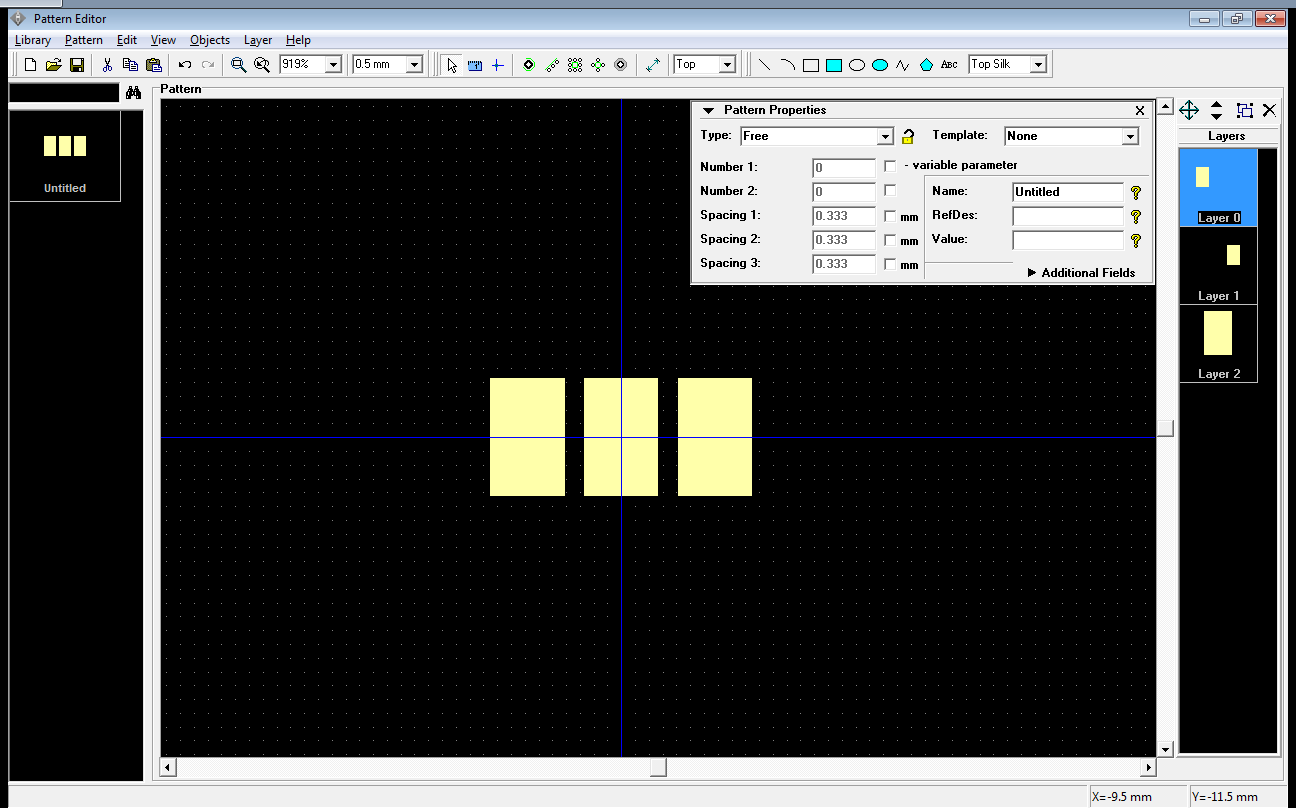
\includegraphics[width=5.4in,height=3.3665in]{figures/ee4document-img038.png} \newline
The pads are numbered from left to right as follows: 1, 3, 2}

{\selectlanguage{english}\sffamily\color[rgb]{0.30980393,0.5058824,0.7411765}
Now, repeat for the center heatsink pad. If you set up the origin as defined above, you should get 

\includegraphics[width=0.3854in,height=0.2083in]{figures/ee4document-img039.png}  for the pad position, 1.1mm for the width,
and 3.9mm for the height. Since this pad's dimensions are not consistent with the rest of the pattern, you will want to
uncheck {\textquotedbl}Use Pattern's Pad Properties{\textquotedbl} and enter custom properties.}

\liststyleRTFNumxi
\setcounter{saveenum}{\value{enumi}}
\begin{enumerate}
\setcounter{enumi}{\value{saveenum}}
\item {\selectlanguage{english}\sffamily\color[rgb]{0.30980393,0.5058824,0.7411765}
Add a polarity indicator. If you look at the LED's mechanical drawing, you will see a chamfer on the cathode side. Add a
silkscreen dot on the pattern by drawing a circle. Adjust the circle parameters to your liking.}
\item {\selectlanguage{english}\sffamily\color[rgb]{0.30980393,0.5058824,0.7411765}
Give your component a name and refdes letter. Since this is a LED, use D for the refdes letter.\newline
 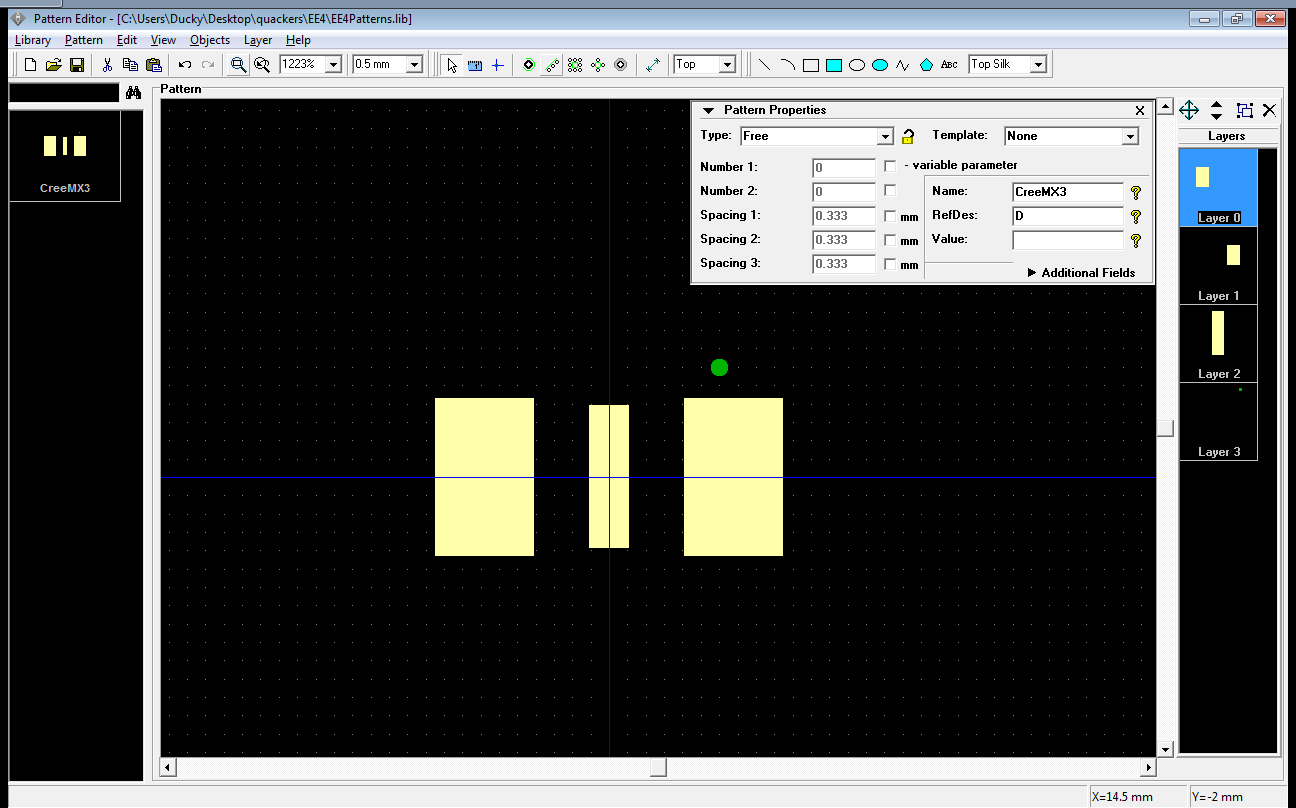
\includegraphics[width=5.4in,height=3.3665in]{figures/ee4document-img040.png} }
\end{enumerate}
{\selectlanguage{english}\sffamily\color[rgb]{0.30980393,0.5058824,0.7411765}
You can also add dimensions (using the Place Dimension button on the toolbar) to compare your pattern with the
datasheet. Dimension edges will automatically snap to relevant features like pad edges and centers.\newline
 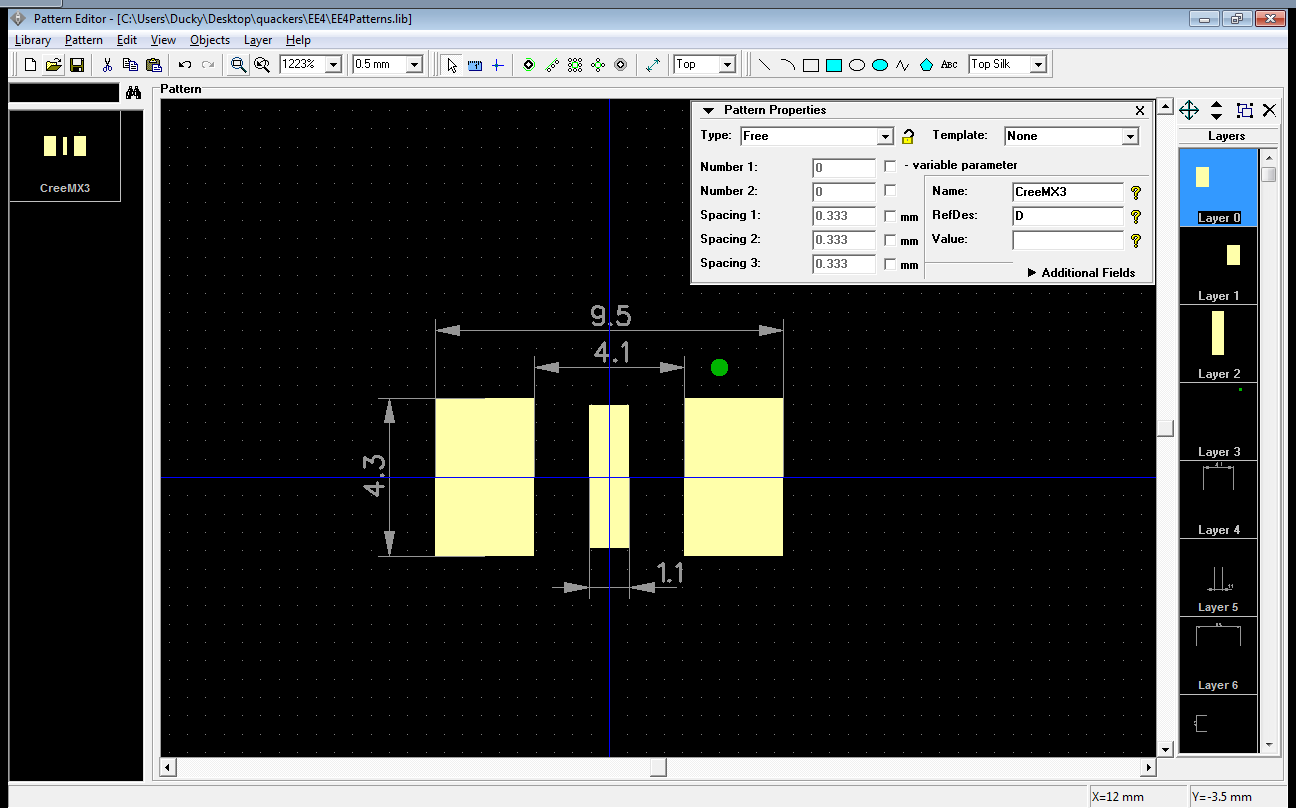
\includegraphics[width=5.4in,height=3.3665in]{figures/ee4document-img041.png} \newline
}

\subsubsection{Component creation}
\hypertarget{Toc337742704}{}{\selectlanguage{english}\sffamily\color[rgb]{0.30980393,0.5058824,0.7411765}
You have a pattern, now you need a schematic symbol.}


\bigskip

{\selectlanguage{english}\sffamily\color[rgb]{0.30980393,0.5058824,0.7411765}
Start the DipTrace component editor.\newline
 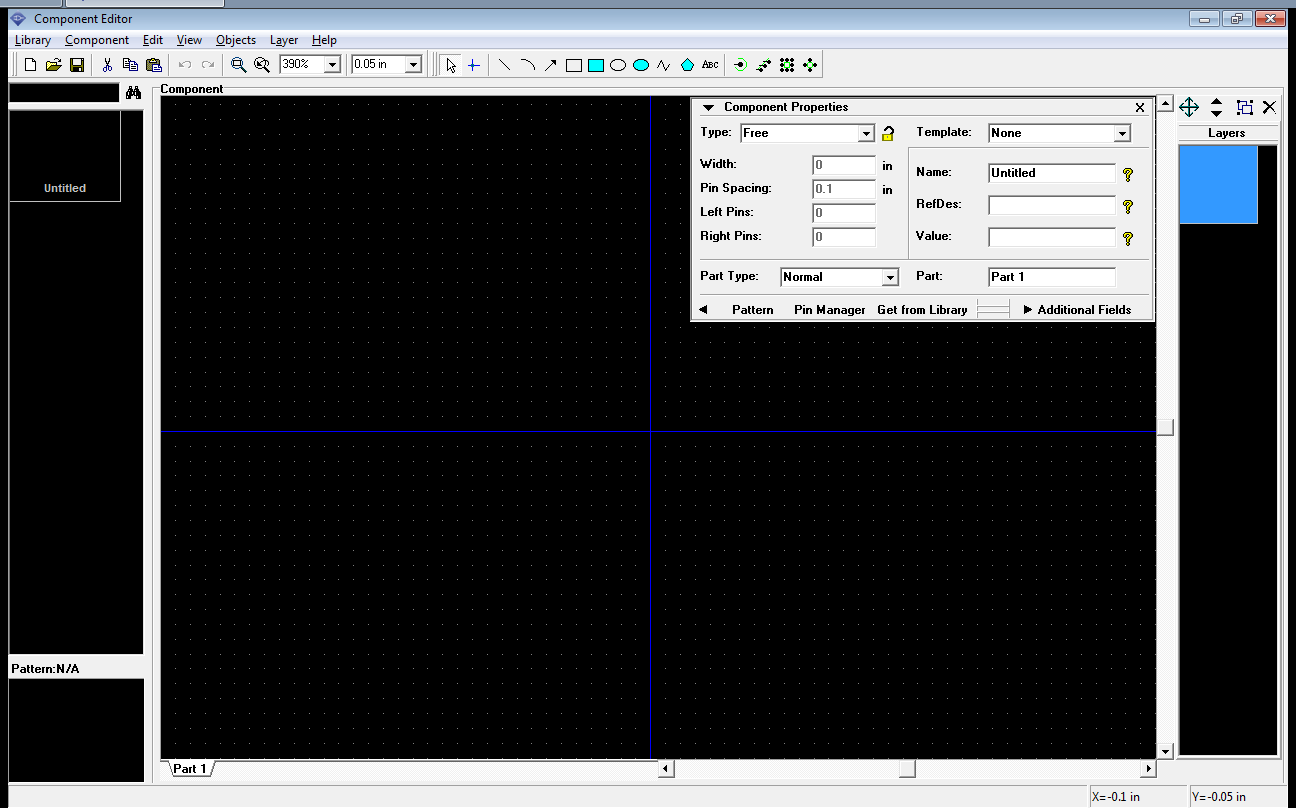
\includegraphics[width=5.4in,height=3.3665in]{figures/ee4document-img042.png} }

{\selectlanguage{english}\sffamily\color[rgb]{0.30980393,0.5058824,0.7411765}
Often, it's easier to base your part off an existing schematic symbol, especially for complex parts like LEDs.}

\liststyleRTFNumxi
\setcounter{saveenum}{\value{enumi}}
\begin{enumerate}
\setcounter{enumi}{\value{saveenum}}
\item \setcounter{saveenum}{\value{enumii}}
\begin{enumerate}
\setcounter{enumii}{\value{saveenum}}
\item {\selectlanguage{english}\sffamily\color[rgb]{0.30980393,0.5058824,0.7411765}
Open the existing {\textquotedbl}discrete.eli{\textquotedbl} library.}
\item {\selectlanguage{english}\sffamily\color[rgb]{0.30980393,0.5058824,0.7411765}
Select {\textquotedbl}LED{\textquotedbl} from the list of patterns. It should open in the main view.}
\item {\selectlanguage{english}\sffamily\color[rgb]{0.30980393,0.5058824,0.7411765}
Select all (Ctrl+A) and copy (Ctrl+C).}
\end{enumerate}
\item {\selectlanguage{english}\sffamily\color[rgb]{0.30980393,0.5058824,0.7411765}
Create a new library by clicking Library-{\textgreater}New.}
\end{enumerate}
{\selectlanguage{english}\sffamily\color[rgb]{0.30980393,0.5058824,0.7411765}
Paste the copied LED schematic. Note that, for whatever reason, the schematic is not aligned. Nudge it up and to the
right by 0.031 in. A simple way to do this is to set the grid to 0.031 in, select everything, and hit the up arrow and
right arrow once.\newline
 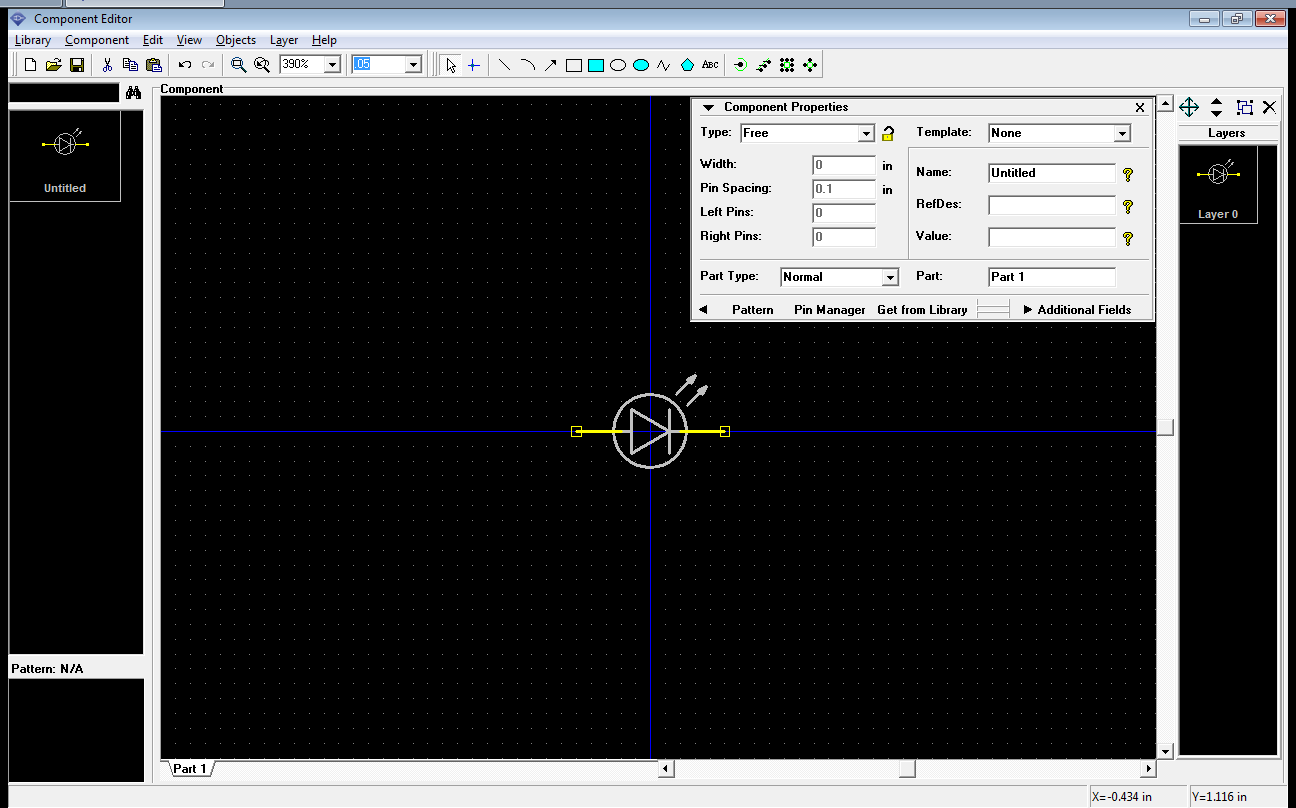
\includegraphics[width=5.4in,height=3.3665in]{figures/ee4document-img043.png} }

{\selectlanguage{english}\sffamily\color[rgb]{0.30980393,0.5058824,0.7411765}
The original LED has only two pins: anode and cathnode. However, we also have a heatsink pin. Click the
{\textquotedbl}Pin{\textquotedbl} button on the toolbox and add a new pin.\newline
 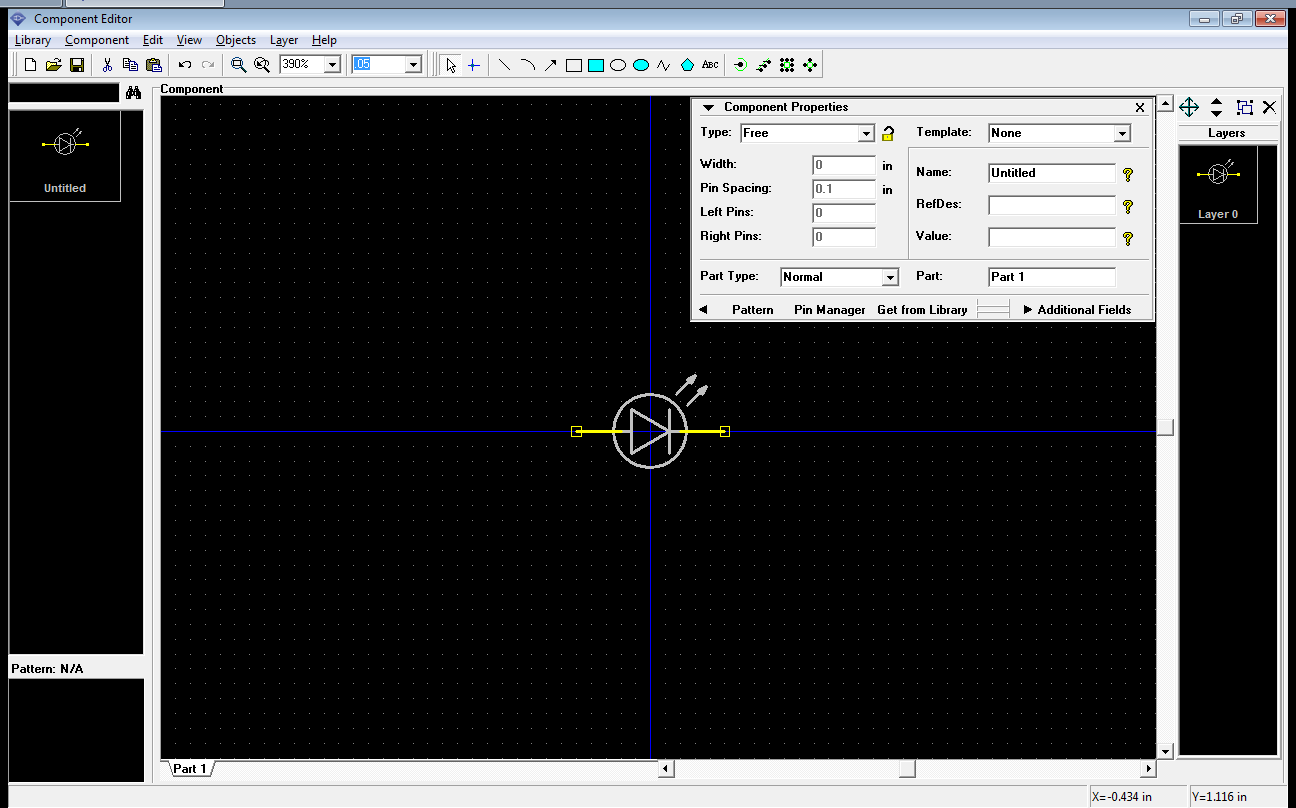
\includegraphics[width=0.9402in,height=0.252in]{figures/ee4document-img043.png} \newline
Position the pin such that it is below the LED and faces downward. You can rotate components by using the right click
menu, or pressing Ctrl+R.\newline
 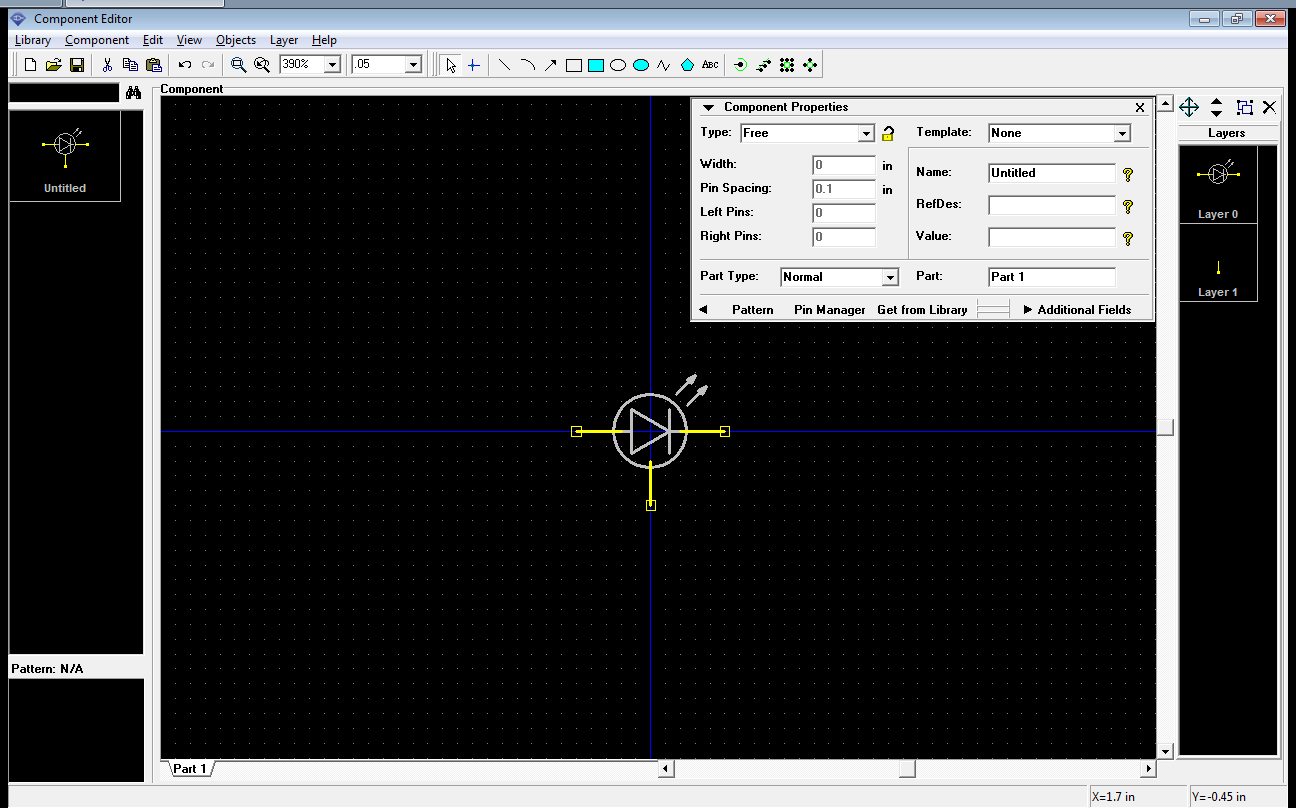
\includegraphics[width=5.4in,height=3.3665in]{figures/ee4document-img044.png} }

{\selectlanguage{english}\sffamily\color[rgb]{0.30980393,0.5058824,0.7411765}
Go into the Pin Manager and define the new pin:\newline
 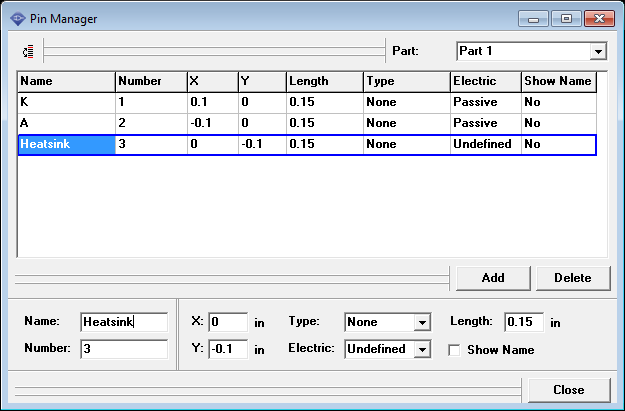
\includegraphics[width=2.6043in,height=1.7126in]{figures/ee4document-img045.png} \newline
Here is where you can also activate the {\textquotedbl}Show Name{\textquotedbl} option for each pin. Experiment with it.
Although not particularly useful for a LED, this is invaluable on chips.}

{\selectlanguage{english}\sffamily\color[rgb]{0.30980393,0.5058824,0.7411765}
Go into the Pattern dialog and define the associated pattern (what you just created before.) You will need to load your
pattern library by using the {\textquotedbl}Add{\textquotedbl} button.\newline
 \includegraphics[width=2.1165in,height=2.6457in]{figures/ee4document-img046.png} \newline
Ensure that the pins match as expected.}

{\selectlanguage{english}\sffamily\color[rgb]{0.30980393,0.5058824,0.7411765}
Give your component a name and refdes letter.\newline
 \includegraphics[width=5.4in,height=3.3665in]{figures/ee4document-img047.png} }

\subsubsection{Revising the schematic}
\hypertarget{Toc337742705}{}{\selectlanguage{english}\sffamily\color[rgb]{0.30980393,0.5058824,0.7411765}
You build the component, now put it into your schematic.}


\bigskip

\liststyleRTFNumxi
\setcounter{saveenum}{\value{enumi}}
\begin{enumerate}
\setcounter{enumi}{\value{saveenum}}
\item {\selectlanguage{english}\sffamily\color[rgb]{0.30980393,0.5058824,0.7411765}
Remove the old LED in your schematic and add your new one.}
\end{enumerate}
{\selectlanguage{english}\sffamily\color[rgb]{0.30980393,0.5058824,0.7411765}
You may also want to scale down the resistor to the LED. If the input voltage was 5v\footnote{\ The CR2032 battery in
the holder actually runs at around 3.0v, but that's not even enough voltage to overcome the forward voltage drop of the
high-power LED.} and you wanted to run the LED at 150 mA, the resistor would be set at 
\includegraphics[width=1.0311in,height=8.9984in]{figures/ee4document-img048.png} .}

{\selectlanguage{english}\sffamily\color[rgb]{0.30980393,0.5058824,0.7411765}
There is the issue of the Heatsink pad. We will not electrically connect it\footnote{\ A heatsink does not need to be
electrically connected, but it should be connected to a large area of copper to help dissipate heat. Typically,
heatsinks can be electrically connected to ground. This is especially useful if your board has a ground plane. You
should double check the datasheet to see if a heatsink pin is internally connected anywhere.}, so right click the pin
and select {\textquotedbl}Not connected.{\textquotedbl} This is typically good practice as it eliminates any ambiguity
as to whether a pin is intentionally not connected, or left unconnected by mistake.\newline
\newline
 \includegraphics[width=5.4in,height=3.3665in]{figures/ee4document-img049.png} }

\subsubsection{Revising the board}
\hypertarget{Toc337742706}{}\liststyleRTFNumxi
\setcounter{saveenum}{\value{enumi}}
\begin{enumerate}
\setcounter{enumi}{\value{saveenum}}
\item {\selectlanguage{english}\sffamily\color[rgb]{0.30980393,0.5058824,0.7411765}
Forward annotate your schematic modifications to your PCB layout.}
\item {\selectlanguage{english}\sffamily\color[rgb]{0.30980393,0.5058824,0.7411765}
By default, DipTrace snaps components to the grid based on the center of their Pin 1. This works well for through-hole
components, but can cause strange behavior for surface-mount components whose dimensions aren't always a multiple of
100mil. Right click the new LED and choose Snap to Grid-{\textgreater}By Origin.}
\end{enumerate}
{\selectlanguage{english}\sffamily\color[rgb]{0.30980393,0.5058824,0.7411765}
Route your new component.\newline
 \includegraphics[width=5.4in,height=3.3665in]{figures/ee4document-img050.png} }

{\selectlanguage{english}\sffamily\color[rgb]{0.30980393,0.5058824,0.7411765}
You're done. You can re-export Gerbers if you want the extra practice.}

\section{Design Software}
\hypertarget{Toc337742707}{}{\selectlanguage{english}\sffamily\color[rgb]{0.30980393,0.5058824,0.7411765}
CalSol uses DipTrace, however, there are more. A brief listing follows (for a more complete listing, see Wikipedia:
\url{https://en.wikipedia.org/wiki/Comparison_of_EDA_software}):}

\subsection{Free \& Open Source}
\hypertarget{Toc337742708}{}{\selectlanguage{english}\sffamily\color[rgb]{0.30980393,0.5058824,0.7411765}
In general, free \& open source software, especially in the niche EDA area, is less well-developed than their commercial
counterparts. However, they are definitely viable, and you do have the advantage of getting access to the source code
and there is no risk of vendor lock-in or ridiculous DRM schemes.}

\liststyleRTFNumxii
\begin{itemize}
\item {\selectlanguage{english}\sffamily\color[rgb]{0.30980393,0.5058824,0.7411765}
gEDA and PCB - a GPL-licensed board design suite.}
\item {\selectlanguage{english}\sffamily\color[rgb]{0.30980393,0.5058824,0.7411765}
KiCAD -- another GPL-licensed board design suite.}
\end{itemize}
\subsection{Commercial}
\hypertarget{Toc337742709}{}\subsubsection{Software you can afford}
\hypertarget{Toc337742710}{}{\selectlanguage{english}\sffamily\color[rgb]{0.30980393,0.5058824,0.7411765}
Hobbyist-grade and above. Most have free trial versions, either time-limited to pin-limited.}

\liststyleRTFNumxii
\begin{itemize}
\item {\selectlanguage{english}\sffamily\color[rgb]{0.30980393,0.5058824,0.7411765}
DipTrace - what CalSol uses.}
\item {\selectlanguage{english}\sffamily\color[rgb]{0.30980393,0.5058824,0.7411765}
EAGLE - pretty much the hobbyist standard, but has unpleasant
DRM\footnote{\ \url{https://groups.google.com/forum/?fromgroups=\#!topic/comp.arch.embedded/95ToLSa1nhg} }.}
\end{itemize}
\subsubsection{Software for the 1\%}
\hypertarget{Toc337742711}{}{\selectlanguage{english}\sffamily\color[rgb]{0.30980393,0.5058824,0.7411765}
You probably can't afford it. However, businesses are willing to put down the dough for the features and support
offered. In some cases, the software may even replace a human board designer, which can save the company serious
money.}

\liststyleRTFNumxii
\begin{itemize}
\item {\selectlanguage{english}\sffamily\color[rgb]{0.30980393,0.5058824,0.7411765}
Altium Designer}
\item {\selectlanguage{english}\sffamily\color[rgb]{0.30980393,0.5058824,0.7411765}
Cadence Allegro, Cadence OrCAD}
\item {\selectlanguage{english}\sffamily\color[rgb]{0.30980393,0.5058824,0.7411765}
Mentor Graphics PowerPCB}
\end{itemize}
\clearpage
\bigskip

\section{PCBs and You}
\hypertarget{Toc337742712}{}{\selectlanguage{english}\sffamily\color[rgb]{0.30980393,0.5058824,0.7411765}
CalSol gets its circuit board manufacturing sponsored by Advanced Circuits. However, there are many board houses out
there, each with its advantages and disadvantages. A brief listing follows of places you can get one-of boards
relatively cheaply. If you are looking for volume production, you will have many more options.}

\subsection{Advanced Circuits}
\hypertarget{Toc337742713}{}{\selectlanguage{english}\sffamily\color[rgb]{0.30980393,0.5058824,0.7411765}
\href{http://www.4pcb.com/}{\textcolor{blue}{http://www.4pcb.com}} }

{\selectlanguage{english}\sffamily\color[rgb]{0.30980393,0.5058824,0.7411765}
Advanced Circuits is a US-based commercial board house. They are more focused towards business customers and volume
production, but do have a special student offer.}

{\selectlanguage{english}\sffamily\color[rgb]{0.30980393,0.5058824,0.7411765}
\url{http://www.4pcb.com/index.php?load=content&page_id=134} }

\liststyleRTFNumxv
\begin{itemize}
\item {\selectlanguage{english}\sffamily\color[rgb]{0.30980393,0.5058824,0.7411765}
Turn-around: 5 days, then shipping}
\item {\selectlanguage{english}\sffamily\color[rgb]{0.30980393,0.5058824,0.7411765}
Design rules: 2 layers, 6mil/6mil trace width/spacing, 15mil minimum drill}
\item {\selectlanguage{english}\sffamily\color[rgb]{0.30980393,0.5058824,0.7411765}
Cost: \$33 each, maximum board size is 60 sq in}
\item {\selectlanguage{english}\sffamily\color[rgb]{0.30980393,0.5058824,0.7411765}
Many other options available at different pricing structures}
\end{itemize}
\subsection{BatchPCB}
\hypertarget{Toc337742714}{}{\selectlanguage{english}\sffamily\color[rgb]{0.30980393,0.5058824,0.7411765}
\url{http://batchpcb.com/} }

{\selectlanguage{english}\sffamily\color[rgb]{0.30980393,0.5058824,0.7411765}
BatchPCB is a SparkFun PCB service. They take peoples orders and combine them onto one order, which they send out to
manufacture.}

\liststyleRTFNumxvii
\begin{itemize}
\item {\selectlanguage{english}\sffamily\color[rgb]{0.30980393,0.5058824,0.7411765}
Turn-around: about 2-3 weeks}
\item {\selectlanguage{english}\sffamily\color[rgb]{0.30980393,0.5058824,0.7411765}
Design rules: 2 layers, 8mil/8mil trace width/spacing, 20mil minimum drill}
\item {\selectlanguage{english}\sffamily\color[rgb]{0.30980393,0.5058824,0.7411765}
Cost: \$2.50 per sq. in., plus \$10 setup fee}
\item {\selectlanguage{english}\sffamily\color[rgb]{0.30980393,0.5058824,0.7411765}
4 layer boards also available, for an additional fee}
\end{itemize}
\subsection{Dorkbot PDX / OSH Park}
\hypertarget{Toc337742715}{}{\selectlanguage{english}\sffamily\color[rgb]{0.30980393,0.5058824,0.7411765}
\url{http://oshpark.com/} }

\liststyleRTFNumiv
\begin{itemize}
\item {\selectlanguage{english}\sffamily\color[rgb]{0.30980393,0.5058824,0.7411765}
Turn-around: about 2 weeks}
\item {\selectlanguage{english}\sffamily\color[rgb]{0.30980393,0.5058824,0.7411765}
Design rules: 6mil/6mil trace width/spacing, 13 mil minimum drill}
\item {\selectlanguage{english}\sffamily\color[rgb]{0.30980393,0.5058824,0.7411765}
2-layer cost: \$5 per sq. in., you get 3 copes}
\item {\selectlanguage{english}\sffamily\color[rgb]{0.30980393,0.5058824,0.7411765}
4-layer cost: \$10 per sq. in., you get 3 copies}
\end{itemize}
\subsection{SeeedStudio}
\hypertarget{Toc337742716}{}{\selectlanguage{english}\sffamily\color[rgb]{0.30980393,0.5058824,0.7411765}
\url{http://www.seeedstudio.com/depot/fusion-pcb-service-p-835.html?cPath=185} }

\liststyleRTFNumiii
\begin{itemize}
\item {\selectlanguage{english}\sffamily\color[rgb]{0.30980393,0.5058824,0.7411765}
Turn-around: about 1 week for manufacturing, then shipping from China}
\item {\selectlanguage{english}\sffamily\color[rgb]{0.30980393,0.5058824,0.7411765}
Design rules: 2 layers, 6mil/6mil trace width/spacing, 0.3mm minimum drill}
\item {\selectlanguage{english}\sffamily\color[rgb]{0.30980393,0.5058824,0.7411765}
Cost: \$9.90 for 10 copies of a 5cm x 5cm board, other sizes also available}
\end{itemize}

\bigskip

{\selectlanguage{english}\sffamily\color[rgb]{0.30980393,0.5058824,0.7411765}
... and many others - Google if you are truly interested ...}

\section{Sources \& Further Reading}
\hypertarget{Toc337742717}{}{\selectlanguage{english}\sffamily\color[rgb]{0.30980393,0.5058824,0.7411765}
\textstyleSubtleEmphasis{These references were used in the creation of this document. If you want to learn more, take a
look at these sites!}}


\bigskip

{\selectlanguage{english}\sffamily\color[rgb]{0.30980393,0.5058824,0.7411765}
\url{https://en.wikipedia.org/wiki/Printed_circuit_board}}

{\selectlanguage{english}\sffamily\color[rgb]{0.30980393,0.5058824,0.7411765}
\url{https://en.wikipedia.org/wiki/Schematic_capture}}

{\selectlanguage{english}\sffamily\color[rgb]{0.30980393,0.5058824,0.7411765}
\url{http://www.alternatezone.com/electronics/files/PCBDesignTutorialRevA.pdf} - contains many good tips on board
layout}

{\selectlanguage{english}\sffamily\color[rgb]{0.30980393,0.5058824,0.7411765}
\url{http://batchpcb.com/index.php/Faq}}


\bigskip
\end{document}
